% !TEX program = pdflatex
% Build from this folder:  latexmk -pdf n_qubit_simulator_tutorial.tex
% Figures and numbers:     python make_tutorial_figures.py  (run from fourqubitv5)
\documentclass[11pt,a4paper]{article}

\usepackage[T1]{fontenc}
\usepackage[utf8]{inputenc}
\usepackage{lmodern}
\usepackage{textcomp}
\usepackage{amsmath,amssymb,mathtools}
\usepackage{braket}
\usepackage[a4paper,margin=2.2cm]{geometry}
\usepackage{graphicx}
\usepackage[dvipsnames]{xcolor}
\usepackage{booktabs,tabularx,array,multirow,makecell}
\usepackage{enumitem}
\usepackage{listings}
\usepackage[most]{tcolorbox}
\usepackage{tikz}
\usetikzlibrary{mindmap,trees,positioning,arrows.meta,shapes.geometric,shapes.multipart,fit,backgrounds,calc,decorations.pathreplacing}
\usepackage[edges]{forest}
\usepackage{dirtree}
\usepackage{caption}
\captionsetup{font=small,labelfont=bf}
\usepackage{float}
\usepackage{microtype}
\usepackage[colorlinks=true,linkcolor=blue!50!black,citecolor=OliveGreen,urlcolor=blue!60!black]{hyperref}
\usepackage[nameinlink,capitalise]{cleveref}

\emergencystretch=3em
\setlength{\parskip}{0.45em}
\setlength{\parindent}{0pt}
\setlist{itemsep=0.15em,topsep=0.3em}

\DeclareRobustCommand{\code}[1]{\texttt{\detokenize{#1}}}
\newcommand{\ad}{a^{\dagger}}
\newcommand{\Tr}{\operatorname{Tr}}
\newcommand{\MHz}{\,\mathrm{MHz}}
\newcommand{\kHz}{\,\mathrm{kHz}}
\newcommand{\GHz}{\,\mathrm{GHz}}
\newcommand{\ns}{\,\mathrm{ns}}
\newcommand{\us}{\,\mu\mathrm{s}}
\newcommand{\hc}{\text{h.c.}}
\newcommand{\eqlab}[1]{\refstepcounter{equation}\tag{\theequation}\label{#1}}

\lstdefinestyle{py}{
  language=Python,
  basicstyle=\ttfamily\footnotesize,
  keywordstyle=\color{RoyalBlue}\bfseries,
  commentstyle=\color{OliveGreen}\itshape,
  stringstyle=\color{BrickRed},
  numbers=left, numberstyle=\tiny\color{gray}, numbersep=6pt, xleftmargin=2.2em,
  frame=single, framerule=0.3pt, rulecolor=\color{gray!50},
  backgroundcolor=\color{gray!4},
  breaklines=true, columns=fullflexible, keepspaces=true,
  showstringspaces=false, tabsize=4, upquote=true, extendedchars=true,
  literate={π}{{\ensuremath{\pi}}}1 {†}{{\ensuremath{^\dagger}}}1 {²}{{\ensuremath{^2}}}1 {×}{{\ensuremath{\times}}}1 {Σ}{{\ensuremath{\Sigma}}}1,
}
\lstset{style=py}
% \src{path relative to n_qubit_simulator}{first line}{last line}
\newcommand{\src}[3]{\lstinputlisting[firstline=#2,lastline=#3,firstnumber=#2,title={\footnotesize\code{#1}, lines #2 to #3}]{../../#1}}

\newtcolorbox{keybox}[1][Key idea]{enhanced,breakable,colback=blue!3,colframe=blue!45!black,fonttitle=\bfseries\small,title={#1},left=5pt,right=5pt,top=3pt,bottom=3pt}
\newtcolorbox{warnbox}[1][Watch out]{enhanced,breakable,colback=red!3,colframe=red!55!black,fonttitle=\bfseries\small,title={#1},left=5pt,right=5pt,top=3pt,bottom=3pt}
\newtcolorbox{readbox}[1][Read this]{enhanced,breakable,colback=green!3,colframe=green!40!black,fonttitle=\bfseries\small,title={#1},left=5pt,right=5pt,top=3pt,bottom=3pt}
\newtcolorbox{codebox}[1][In the code]{enhanced,breakable,colback=orange!4,colframe=orange!60!black,fonttitle=\bfseries\small,title={#1},left=5pt,right=5pt,top=3pt,bottom=3pt}

\begin{document}

\begin{titlepage}
\centering
\vspace*{2.2cm}
{\Huge\bfseries Inside the n-qubit simulator\par}
\vspace{0.7cm}
{\Large An X-ray of the code, the physics behind every line,\\[0.2em] and where the micro-oscillations come from\par}
\vspace{1.4cm}
{\large\code{fourqubitv5/HM/simulator/n_qubit_simulator}\par}
\vspace{0.5cm}
{\large 10 October 2026\par}
\vfill
\begin{minipage}{0.86\textwidth}\small
This tutorial describes the code exactly as it stands in the repository on the date above. Code listings are pulled
straight from the source files with their real line numbers, so if the code changes, recompiling this document shows the
new lines. Every number quoted in the text is produced by \code{make_tutorial_figures.py} (same folder), which also
writes \code{tutorial_numbers.json}. The physics chapters give exact references so you can read further. Where the
code and the physics can disagree with your intuition, there is a red box.
\end{minipage}
\vspace{1.5cm}
\end{titlepage}

\tableofcontents
\newpage

%=====================================================================
\section*{How to use this document}
\addcontentsline{toc}{section}{How to use this document}

There are three questions behind this document, and each has its own part.

\begin{enumerate}[label=\textbf{\arabic*.}]
\item \textbf{What exactly is coded up?} Part~\ref{part:code} opens every file, shows the real code, and draws the
  structure as mind maps, data-flow diagrams, class diagrams, and call trees. After it you should be able to say, for
  any line of the engine, what physical term it adds and where its numbers come from.
\item \textbf{What is the physics?} Part~\ref{part:physics} derives every term of the Hamiltonian the engine builds,
  starting from the transmon circuit. It ends each topic with a green ``Read this'' box listing exact sources.
\item \textbf{Why are there micro-oscillations in the Bloch plots?} Part~\ref{part:micro} answers this with
  derivations and with dedicated simulations that isolate each cause.
\end{enumerate}

Part~\ref{part:reading} is an ordered reading list. If you only have one evening, read
\cref{sec:onepage,sec:engine,sec:frames,sec:micro-what,sec:micro-drive}.

\begin{keybox}[Conventions used everywhere in this document]
\begin{itemize}
\item \(\hbar = 1\). Frequencies \(f\) are in MHz and times \(t\) in \(\mu\)s, so \(2\pi f t\) is a phase in radians.
  The code multiplies every frequency by \code{TWOPI}, so its Hamiltonian is in rad/\(\mu\)s. When I want numbers in MHz I
  write \(H/2\pi\).
\item Kets list qubits in increasing ID order: \(\ket{n_1 n_2 n_3}\) means Q1 in \(n_1\), Q2 in \(n_2\), Q3 in \(n_3\).
\item Transmon anharmonicities are negative: \(\alpha < 0\). The code stores \(-|\alpha|\).
\item Bloch components of one qubit come from its reduced density matrix \(\rho\) restricted to levels 0 and 1:
  \(X = 2\,\mathrm{Re}\,\rho_{01}\), \(Y = -2\,\mathrm{Im}\,\rho_{01}\), \(Z = \rho_{00} - \rho_{11}\). So \(Z=+1\) is \(\ket{0}\).
\item A drive detuning is \(\delta = f_{\text{carrier}} - f_{\text{frame}}\). An edge detuning is
  \(\Delta_{ij} = f_i - f_j\).
\item Q1 is the control and Q2 the target of the c1t2 cross-resonance (CR) gate. Q3 is a spectator coupled to Q2.
\end{itemize}
\end{keybox}

%=====================================================================
\part{The code, X-rayed}\label{part:code}
%=====================================================================

\section{The whole simulator on one page}\label{sec:onepage}

In one sentence: \emph{the simulator integrates the Schr\"odinger equation
\(i\,\tfrac{d}{dt}\ket{\psi(t)} = H(t)\ket{\psi(t)}\) for a few truncated transmons, in a frame that rotates with each
qubit, where \(H(t)\) is assembled from a device description (frequencies, anharmonicities, couplings) and a set of
sampled pulse envelopes, one per drive channel.}

Everything else is bookkeeping around that sentence: where the device numbers come from (\cref{sec:device}), how
\(H(t)\) is assembled (\cref{sec:engine}), how pulses become envelopes (\cref{sec:pulses}), how an experiment asks a
question (\cref{sec:experiments}), and how final states are read back (\cref{sec:analysis}).

\begin{figure}[p]
\centering
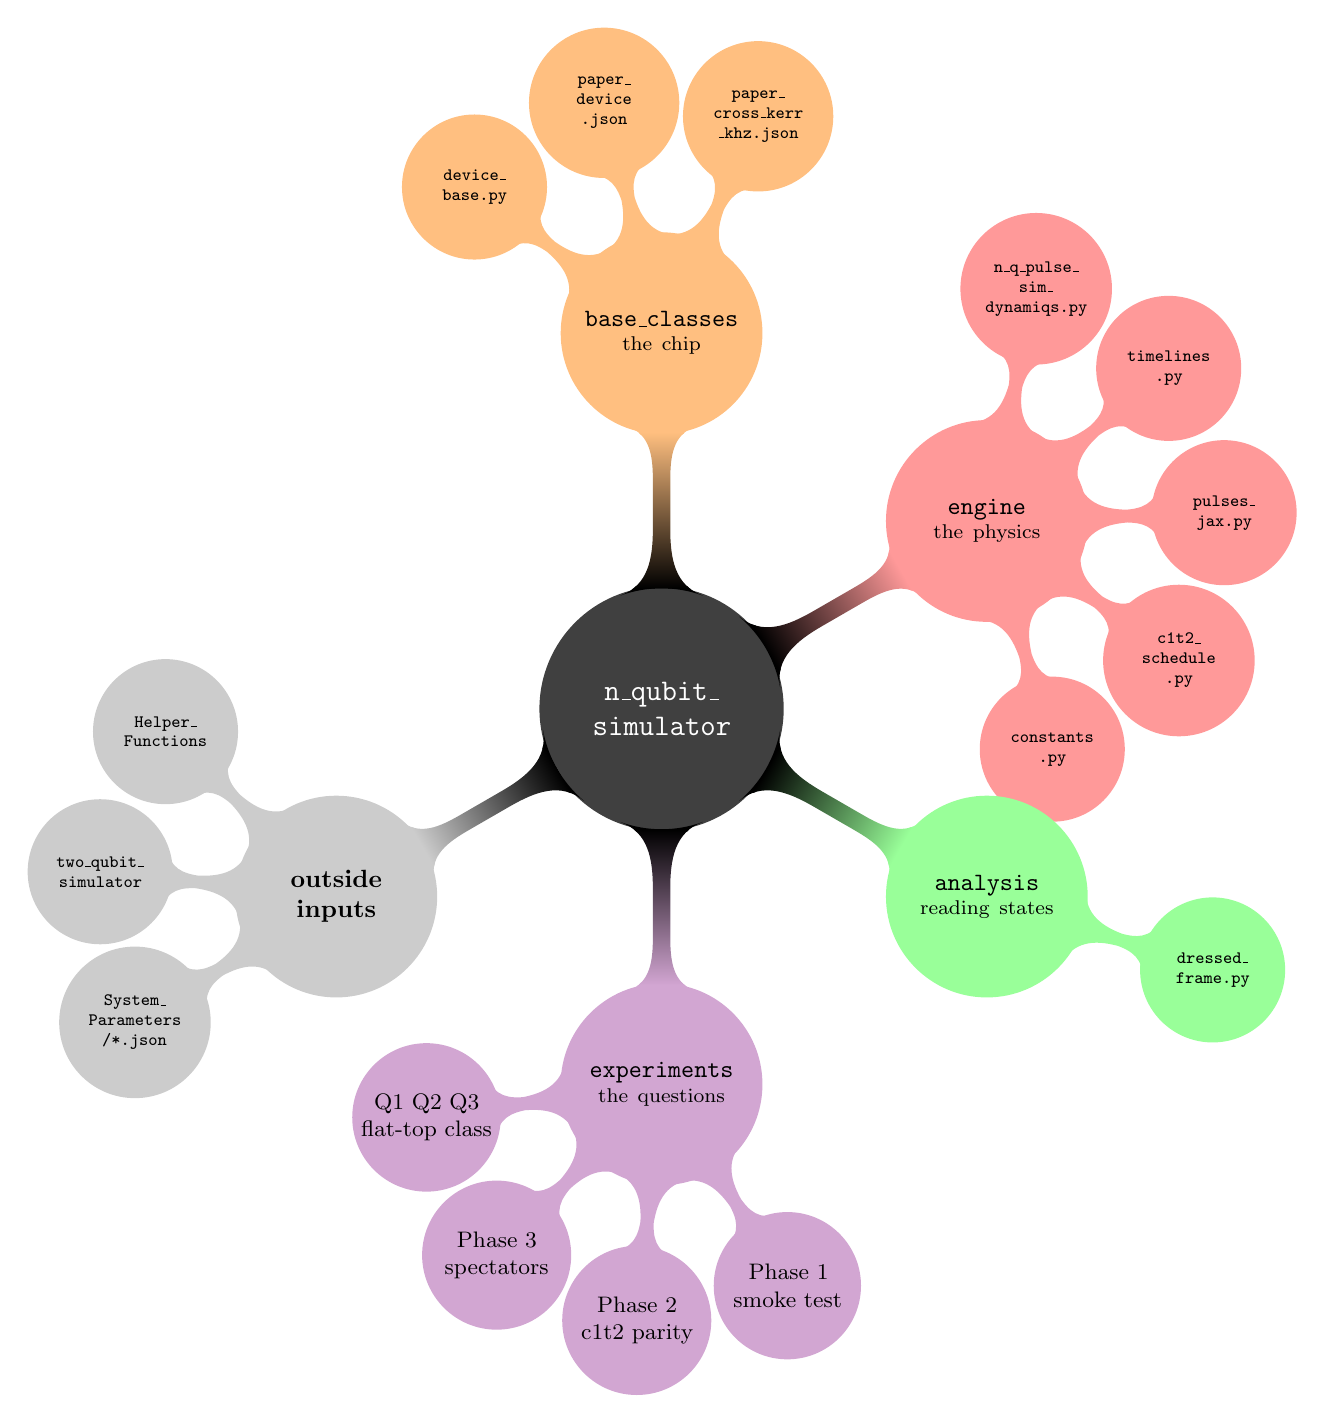
\begin{tikzpicture}[
  mindmap, scale=0.9, transform shape,
  every node/.style={concept, execute at begin node=\hskip0pt},
  root concept/.append style={concept color=black!75, text=white, font=\large\ttfamily\bfseries, minimum size=3.4cm, text width=3cm},
  level 1 concept/.append style={level distance=5.3cm, font=\normalsize\bfseries, minimum size=2.8cm, text width=2.5cm},
  level 2 concept/.append style={level distance=3.35cm, sibling angle=38, font=\small, minimum size=2.0cm, text width=1.85cm},
  file/.style={font=\ttfamily\scriptsize},
  text=black
]
\node [root concept] {n\_qubit\_\\simulator}
  [clockwise from=90, sibling angle=72]
  child [concept color=orange!50] { node {\texttt{base\_classes}\\[-0.2em]{\footnotesize\mdseries the chip}}
    [clockwise from=142]
    child { node[file] {device\_\\base.py} }
    child { node[file] {paper\_\\device\\.json} }
    child { node[file] {paper\_\\cross\_kerr\\\_khz.json} } }
  child [concept color=red!40] { node {\texttt{engine}\\[-0.2em]{\footnotesize\mdseries the physics}}
    [clockwise from=78]
    child { node[file] {n\_q\_pulse\_\\sim\_\\dynamiqs.py} }
    child { node[file] {timelines\\.py} }
    child { node[file] {pulses\_\\jax.py} }
    child { node[file] {c1t2\_\\schedule\\.py} }
    child { node[file] {constants\\.py} } }
  child [concept color=green!40] { node {\texttt{analysis}\\[-0.2em]{\footnotesize\mdseries reading states}}
    [clockwise from=-18]
    child { node[file] {dressed\_\\frame.py} } }
  child [concept color=violet!35] { node {\texttt{experiments}\\[-0.2em]{\footnotesize\mdseries the questions}}
    [clockwise from=-58]
    child { node {Phase 1 smoke test} }
    child { node {Phase 2 c1t2 parity} }
    child { node {Phase 3 spectators} }
    child { node {Q1 Q2 Q3 flat-top class} } }
  child [concept color=gray!40] { node {outside inputs}
    [clockwise from=212]
    child { node[file] {System\_\\Parameters\\/*.json} }
    child { node[file] {two\_qubit\_\\simulator} }
    child { node[file] {Helper\_\\Functions} } };
\end{tikzpicture}
\caption{Mind map of the package. Orange builds the chip, red holds the physics and the pulses, green reads final
states, violet asks questions. Grey nodes are code that lives outside the package but is called by it: the lab
parameter files, the trusted 2Q simulator (for the calibrated flat-top and for the fidelity functions), and the lab
pulse helpers (for the DRAG X\(\pi\) and the rise and fall templates).}
\label{fig:mindmap}
\end{figure}

\begin{figure}[p]
\centering
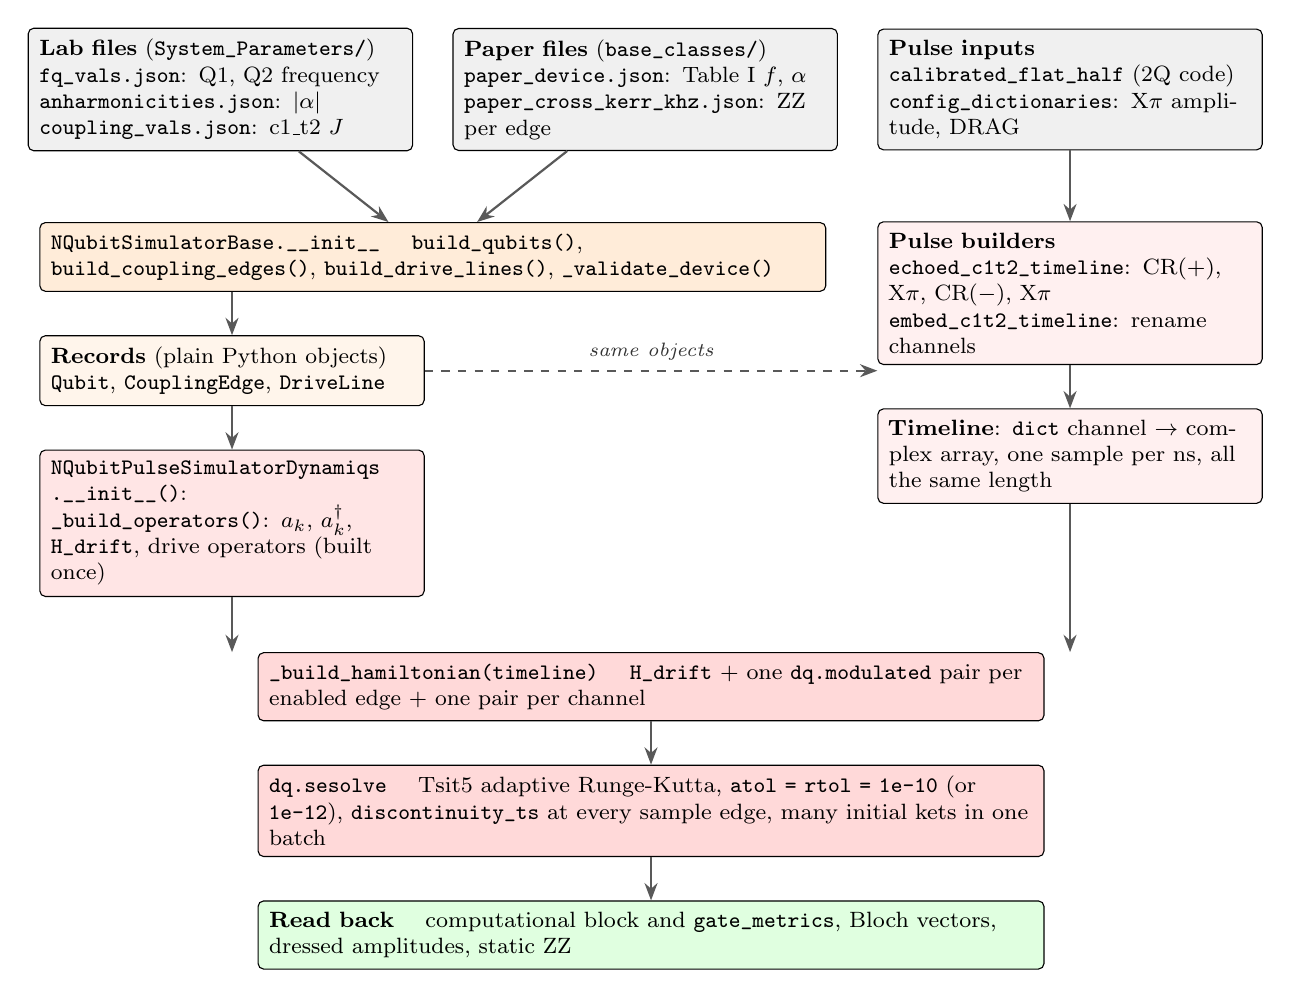
\begin{tikzpicture}[
  node distance=0.55cm and 0.5cm,
  box/.style={draw, rounded corners=2pt, align=left, font=\footnotesize, inner sep=4pt, text width=#1},
  box/.default=5.2cm,
  arr/.style={-{Stealth[length=2.2mm]}, thick, gray!70!black},
  lab/.style={font=\scriptsize\itshape, text=gray!40!black}
]
\node[box=4.6cm, fill=gray!12] (lab) {\textbf{Lab files} (\code{System_Parameters/})\\
\code{fq_vals.json}: Q1, Q2 frequency\\ \code{anharmonicities.json}: \(|\alpha|\)\\ \code{coupling_vals.json}: c1\_t2 \(J\)};
\node[box=4.6cm, fill=gray!12, right=of lab] (paper) {\textbf{Paper files} (\code{base_classes/})\\
\code{paper_device.json}: Table I \(f\), \(\alpha\)\\ \code{paper_cross_kerr_khz.json}: ZZ per edge};
\node[box=4.6cm, fill=gray!12, right=of paper] (pulsein) {\textbf{Pulse inputs}\\
\code{calibrated_flat_half} (2Q code)\\ \code{config_dictionaries}: X\(\pi\) amplitude, DRAG};

\path (lab.south) -- (paper.south) coordinate[midway] (topmid);
\node[box=9.7cm, fill=orange!15, below=0.9cm of topmid] (base) {\textbf{\code{NQubitSimulatorBase.__init__}}
\quad \code{build_qubits()}, \code{build_coupling_edges()}, \code{build_drive_lines()}, \code{_validate_device()}};
\node[box=4.6cm, fill=orange!8, below=of base.south west, anchor=north west] (records) {\textbf{Records} (plain Python objects)\\
\code{Qubit}, \code{CouplingEdge}, \code{DriveLine}};
\node[box=4.6cm, fill=red!10, below=of records] (engine) {\textbf{\code{NQubitPulseSimulatorDynamiqs}}\\ \code{.__init__()}:\\
\code{_build_operators()}: \(a_k\), \(\ad_k\), \code{H_drift}, drive operators (built once)};

\node[box=4.6cm, fill=red!6, below=0.9cm of pulsein] (sched) {\textbf{Pulse builders}\\
\code{echoed_c1t2_timeline}: CR(+), X\(\pi\), CR(\(-\)), X\(\pi\)\\ \code{embed_c1t2_timeline}: rename channels};
\node[box=4.6cm, fill=red!6, below=of sched] (tl) {\textbf{Timeline}: \code{dict} channel \(\to\) complex array, one sample per ns, all the same length};

\path (engine.south) -- (tl.south) coordinate[midway] (lowmid);
\coordinate (hamtop) at (lowmid |- engine.south);
\node[box=9.7cm, fill=red!15, below=0.7cm of hamtop] (ham) {\textbf{\code{_build_hamiltonian(timeline)}} \quad
\code{H_drift} \(+\) one \code{dq.modulated} pair per enabled edge \(+\) one pair per channel};
\node[box=9.7cm, fill=red!15, below=of ham] (solve) {\textbf{\code{dq.sesolve}} \quad Tsit5 adaptive Runge-Kutta, \code{atol = rtol = 1e-10} (or \code{1e-12}),
\code{discontinuity_ts} at every sample edge, many initial kets in one batch};
\node[box=9.7cm, fill=green!12, below=of solve] (ana) {\textbf{Read back} \quad computational block and \code{gate_metrics},
Bloch vectors, dressed amplitudes, static ZZ};

\draw[arr] (lab) -- (base);
\draw[arr] (paper) -- (base);
\draw[arr] (base.south -| records.north) -- (records.north);
\draw[arr] (records) -- (engine);
\draw[arr] (pulsein) -- (sched);
\draw[arr] (sched) -- (tl);
\draw[arr] (engine.south) -- (engine.south |- ham.north);
\draw[arr] (tl.south) -- (tl.south |- ham.north);
\draw[arr] (ham) -- (solve);
\draw[arr] (solve) -- (ana);
\draw[arr, dashed] (records.east) -- node[lab, above, sloped] {same objects} (records.east -| tl.west);
\end{tikzpicture}
\caption{Data flow. Device numbers enter at the top left and become three kinds of records. The engine turns the
records into operators once. Every call to \code{run_shot} or \code{run_shot_batch} then builds a fresh time-dependent
Hamiltonian from the current records and the timeline, and hands it to the solver. The dashed arrow is a reminder that
the engine keeps references to the very same \code{Qubit} and \code{CouplingEdge} objects, so editing a frame or
switching an edge after construction changes the next solve (\cref{tab:rebuild}).}
\label{fig:dataflow}
\end{figure}

\begin{figure}[htbp]
\centering
\begin{minipage}{0.97\textwidth}
\renewcommand*\DTstyle{\ttfamily\footnotesize}
\renewcommand*\DTstylecomment{\rmfamily\footnotesize\color{gray!30!black}}
\DTsetlength{0.2em}{1.6em}{0.2em}{0.4pt}{1.6pt}
\dirtree{%
.1 n\_qubit\_simulator/.
.2 base\_classes/\DTcomment{the chip: records, parameters, provenance}.
.3 device\_base.py\DTcomment{Qubit, DriveLine, CouplingEdge, NQubitSimulatorBase (385 lines)}.
.3 paper\_device.json\DTcomment{paper Table I frequencies and anharmonicities}.
.3 paper\_cross\_kerr\_khz.json\DTcomment{paper static ZZ per edge, used to fit \(J\)}.
.2 engine/\DTcomment{the physics and the pulses}.
.3 n\_q\_pulse\_sim\_dynamiqs.py\DTcomment{Hamiltonian builder and solver call (314 lines)}.
.3 timelines.py\DTcomment{fixed-length per-channel sample buffers}.
.3 pulses\_jax.py\DTcomment{CR half assembly and the echo sequence}.
.3 c1t2\_schedule.py\DTcomment{GRAPE archive loading, the X\(\pi\) builder, channel renaming}.
.3 constants.py\DTcomment{\texttt{TWOPI} and \texttt{DT\_SAMPLE\_NS} = 1 ns}.
.2 analysis/.
.3 dressed\_frame.py\DTcomment{dressed basis, static ZZ, frame compensation}.
.2 experiments/.
.3 closed\_system\_smoke.py\DTcomment{Phase 1: six qutrits, Hermiticity, norm}.
.3 c1t2\_waveform\_identity.py\DTcomment{Phase 2: same samples as the trusted 2Q assembler}.
.3 c1t2\_parity.py\DTcomment{Phase 2: same final states as the 2Q engine}.
.3 spectator\_setup.py\DTcomment{Phase 3: shared chip helpers}.
.3 spectator\_idle\_zz.py\DTcomment{Phase 3: idle ZZ and dressed-frame checks}.
.3 spectator\_gate\_sweep.py\DTcomment{Phase 3: the c1t2 gate with spectators}.
.3 gaussian\_flattop\_fidelity.py\DTcomment{class C1T2FlatFidelity: Q1 Q2 Q3 flat-top}.
.3 results/\DTcomment{JSON outputs}.
.2 documentation/\DTcomment{guides, figures, and this tutorial}.
}
\end{minipage}
\caption{The files, with one line each on what they are for.}
\label{fig:tree}
\end{figure}

%%%%%%%%%%%%%%%%%%%%%%%%%%%%%%%%%%%%%%%%%%%%%%%%%%%%%%%%%%%%%%%%%%%%%%
\section{The device layer: \texorpdfstring{\code{base_classes/device_base.py}}{device\_base.py}}\label{sec:device}

\subsection{Three records}

The whole chip is described by three small dataclasses. They hold numbers and provenance strings and nothing else.

\src{base_classes/device_base.py}{93}{129}

\begin{center}
\small
\begin{tabularx}{\textwidth}{@{}l l X@{}}
\toprule
Record & Field & Meaning \\
\midrule
\code{Qubit} & \code{anharm_MHz} & \(\alpha\), negative, in MHz \\
 & \code{frame_MHz} & frequency of this qubit's rotating frame; in this code it is \emph{also the bare frequency} (\cref{sec:frames}) \\
 & \code{n_levels} & truncation, at least 2 \\
 & \code{f_qubit_MHz} & calibrated frequency; drive carriers are set from it and never move \\
\code{DriveLine} & \code{target_qubit_id} & the qubit whose \(a\) and \(\ad\) this line couples to \\
 & \code{carrier_MHz} & tone frequency; frozen dataclass, cannot change after construction \\
\code{CouplingEdge} & \code{J_MHz} & exchange strength \(J\) in MHz \\
 & \code{enabled} & switch read at every Hamiltonian build \\
 & \code{parameter_source} & where \(J\) came from (\code{coupling_vals.json:...} or \code{paper_zz_fit:...}) \\
\bottomrule
\end{tabularx}
\end{center}

\subsection{The constructor}

\code{NQubitSimulatorBase(qubit_ids, n_levels, levels_by_qubit, dt_sample_ns)} does six things in order:
sorts the requested IDs (tensor order is always Q1 before Q2 before Q3, whatever order you pass), stores the truncation
(with per-qubit overrides), calls \code{build_qubits}, \code{build_coupling_edges}, \code{build_drive_lines},
validates everything, and finally creates the engine and keeps it as \code{self.simulator}.

\src{base_classes/device_base.py}{177}{193}

\subsection{Where every qubit number comes from}

\code{build_qubits} applies one rule: Q1 and Q2 take the lab calibration; Q3 to Q6 take the paper's Table~I values
\cite{deshmukh2026}, with every paper frequency shifted by the same offset
\(f_1^{\text{lab}} - f_1^{\text{paper}} = 5087.614585 - 5031.04 = 56.574585\MHz\), so that detunings relative to Q1 are
those of the paper.

\src{base_classes/device_base.py}{216}{238}

\begin{table}[htbp]
\centering\small
\caption{The model chip as built by \code{NQubitSimulatorBase()} (all six qubits).}
\label{tab:qubits}
\begin{tabular}{@{}c r r l@{}}
\toprule
Qubit & \(f\) (MHz) & \(\alpha\) (MHz) & source string \\
\midrule
Q1 & 5087.614585 & \(-271.2\) & \code{fq_vals.json:1}, \code{anharmonicities.json:1} \\
Q2 & 4983.462676 & \(-266.4\) & \code{fq_vals.json:2}, \code{anharmonicities.json:2} \\
Q3 & 5093.054585 & \(-268.0\) & \code{paper_table_i+q1_offset:3}, \code{paper_table_i:3} \\
Q4 & 5026.174585 & \(-269.0\) & paper plus offset \\
Q5 & 4894.374585 & \(-280.0\) & paper plus offset \\
Q6 & 4981.234585 & \(-271.0\) & paper plus offset \\
\bottomrule
\end{tabular}
\end{table}

\begin{figure}[htbp]
\centering
\includegraphics[width=0.95\textwidth]{figures/frequency_map.pdf}
\caption{Frequency landscape of the model chip. Solid lines are 0-1 transitions, dashed lines 1-2 transitions
(\(f+\alpha\)). The CR tone of c1t2 is applied to Q1 at Q2's frequency (star). Note that Q3 sits 5.4 MHz above Q1
and 109.6 MHz above Q2, and that Q6 sits only 2.2 MHz below Q2, which is why Q6 was the troublesome control-side
spectator in Phase 3.}
\label{fig:freqmap}
\end{figure}

\subsection{Where every coupling comes from}

Edges exist only between odd and even qubits (the chip is the complete bipartite graph \(K_{3,3}\),
\cref{fig:graph}). Only \code{c1_t2} keeps the lab \(J = 3.216328\MHz\). Every other edge gets the \(J\) that
reproduces the paper's measured static ZZ at the paper's own frequencies and anharmonicities. The fit diagonalizes two
5-level transmons exactly (\code{pair_cross_kerr_MHz}) and root-finds \(J\) with Brent's method
(\code{fit_exchange_MHz}).

\src{base_classes/device_base.py}{35}{65}

\begin{figure}[htbp]
\centering
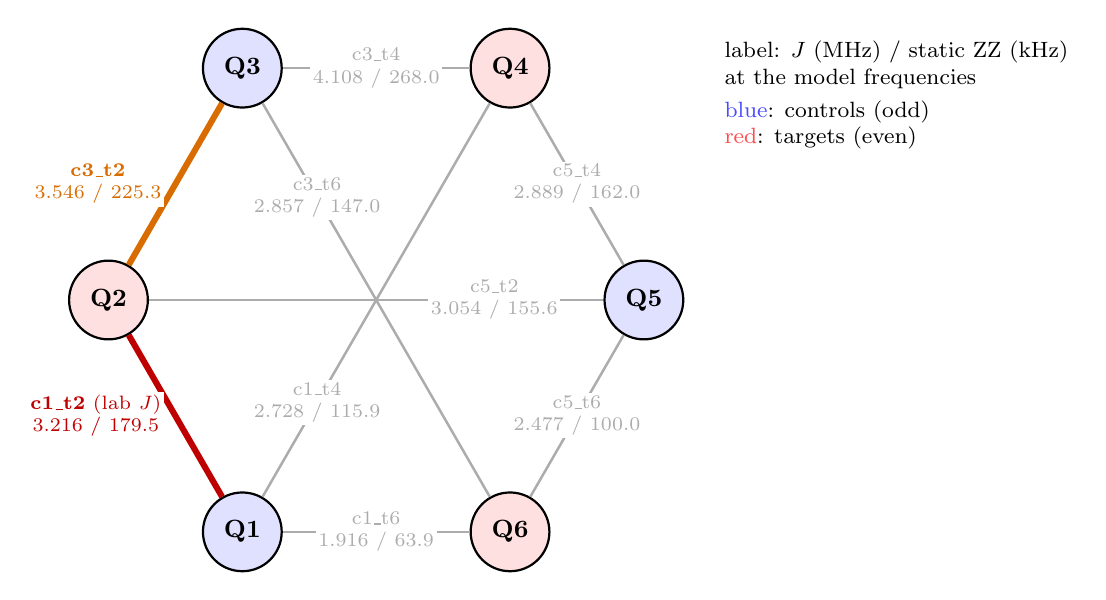
\begin{tikzpicture}[
  q/.style={circle, draw, thick, minimum size=10mm, font=\small\bfseries},
  e/.style={gray!65, line width=0.9pt},
  lab/.style={font=\scriptsize, fill=white, inner sep=1pt, align=center}]
\foreach \q/\ang/\col in {5/0/blue, 4/60/red, 3/120/blue, 2/180/red, 1/240/blue, 6/300/red}
  \node[q, fill=\col!12] (Q\q) at (\ang:3.4) {Q\q};
\draw[e] (Q5) -- node[lab] {c5\_t4\\2.889 / 162.0} (Q4);
\draw[e] (Q4) -- node[lab] {c3\_t4\\4.108 / 268.0} (Q3);
\draw[line width=2.2pt, orange!85!black] (Q3) -- node[lab, left=3pt] {\textbf{c3\_t2}\\3.546 / 225.3} (Q2);
\draw[line width=2.2pt, red!75!black] (Q2) -- node[lab, left=3pt] {\textbf{c1\_t2} (lab \(J\))\\3.216 / 179.5} (Q1);
\draw[e] (Q1) -- node[lab] {c1\_t6\\1.916 / 63.9} (Q6);
\draw[e] (Q6) -- node[lab] {c5\_t6\\2.477 / 100.0} (Q5);
\draw[e] (Q1) -- node[lab, pos=0.24] {c1\_t4\\2.728 / 115.9} (Q4);
\draw[e] (Q3) -- node[lab, pos=0.24] {c3\_t6\\2.857 / 147.0} (Q6);
\draw[e] (Q5) -- node[lab, pos=0.24] {c5\_t2\\3.054 / 155.6} (Q2);
\node[font=\footnotesize, align=left, anchor=west] at (4.3,2.6) {label: \(J\) (MHz) / static ZZ (kHz)\\ at the model frequencies\\[0.3em]
{\color{blue!70}blue}: controls (odd)\\ {\color{red!70}red}: targets (even)};
\end{tikzpicture}
\caption{The coupling graph built by \code{build_coupling_edges}. The two thick edges are the ones on in the Q1 Q2 Q3
experiment. ZZ values are exact two-transmon numbers at the model frequencies of \cref{tab:qubits}.}
\label{fig:graph}
\end{figure}

\subsection{Drive lines}

Every selected qubit gets a self drive \code{q<k>_drive} whose carrier is its own calibrated frequency. Every
selected control-target pair gets a CR line \code{cr_c<c>_t<t>} that acts \emph{on the control} (its
\code{target_qubit_id} is the control) with a carrier at the \emph{target's} frequency. For the Q1 Q2 Q3 chip this
gives five lines:

\begin{center}\small
\begin{tabular}{@{}l c r r@{}}
\toprule
line & acts on & carrier (MHz) & \(\delta =\) carrier \(-\) frame of the qubit it acts on (MHz) \\
\midrule
\code{q1_drive} & Q1 & 5087.614585 & 0 \\
\code{q2_drive} & Q2 & 4983.462676 & 0 \\
\code{q3_drive} & Q3 & 5093.054585 & 0 \\
\code{cr_c1_t2} & Q1 & 4983.462676 & \(-104.151909\) \\
\code{cr_c3_t2} & Q3 & 4983.462676 & \(-109.591909\) \\
\bottomrule
\end{tabular}
\end{center}

\code{_validate_device} then checks the ID order, truncations, unique names, that each edge has provenance, that
\(J \ge 0\), and that the number of lines equals qubits plus edges.

%%%%%%%%%%%%%%%%%%%%%%%%%%%%%%%%%%%%%%%%%%%%%%%%%%%%%%%%%%%%%%%%%%%%%%
\section{The engine: \texorpdfstring{\code{engine/n_q_pulse_sim_dynamiqs.py}}{n\_q\_pulse\_sim\_dynamiqs.py}}\label{sec:engine}

This is the file that contains the physics. It is 314 lines long. Here it is, piece by piece.

\subsection{Global settings at import time}

\src{engine/n_q_pulse_sim_dynamiqs.py}{10}{16}

Double precision matters: the gate errors we care about are \(10^{-3}\) and the solver tolerance is \(10^{-10}\) to
\(10^{-12}\). Single precision has only about 7 significant digits.

\subsection{Constructor}

\src{engine/n_q_pulse_sim_dynamiqs.py}{36}{77}

Things to notice: the drive lines are stored in a \code{dict}, so the channel order is the order of
\code{build_drive_lines}; \code{dims} is the tuple of truncations in tensor order; the solver is Tsit5 with equal
absolute and relative tolerance; states are not saved at intermediate times (\code{save_states=False}), so the
engine returns only the final state.

\subsection{The Hilbert space and how states are indexed}

The joint space is the tensor product of the truncated qubits. For the Q1 Q2 Q3 experiment the truncations are
\code{dims = (4, 4, 3)}, so the dimension is \(4 \times 4 \times 3 = 48\). A basis state \(\ket{n_1 n_2 n_3}\) is stored at a
row-major (``odometer'') index, where the last qubit changes fastest:

\[
\text{index}(n_1, n_2, n_3) = (n_1 \cdot 4 + n_2)\cdot 3 + n_3 .
\]

\src{engine/n_q_pulse_sim_dynamiqs.py}{304}{314}

\begin{center}\small
\begin{tabular}{@{}l c c c c c c c@{}}
\toprule
state & \(\ket{000}\) & \(\ket{001}\) & \(\ket{010}\) & \(\ket{100}\) & \(\ket{110}\) & \(\ket{011}\) & \(\ket{332}\) \\
index & 0 & 1 & 3 & 12 & 15 & 4 & 47 \\
\bottomrule
\end{tabular}
\end{center}

So the four computational states of the gate with Q3 in \(\ket{0}\) sit at indices 0, 3, 12, 15. This is the same
ordering \code{dq.destroy(*dims)} uses, so operators and indices agree.

\subsection{Operators and the drift}

\src{engine/n_q_pulse_sim_dynamiqs.py}{85}{112}

\code{dq.destroy(4, 4, 3)} returns three \(48\times48\) matrices \(a_1 = a\otimes\mathbb{1}\otimes\mathbb{1}\),
\(a_2 = \mathbb{1}\otimes a\otimes\mathbb{1}\), \(a_3 = \mathbb{1}\otimes\mathbb{1}\otimes a\), each with
\(\sqrt{n}\) just above the diagonal of its own factor. The drift is

\[
H_{\text{drift}} = \sum_k 2\pi\,\frac{\alpha_k}{2}\,\ad_k\ad_k a_k a_k
= \sum_k 2\pi\,\frac{\alpha_k}{2}\,\hat n_k(\hat n_k - 1), \eqlab{eq:drift}
\]

which is diagonal: level \(n\) of qubit \(k\) gets \(2\pi\cdot\frac{\alpha_k}{2}n(n-1)\), so \(\ket{2}\) gets
\(2\pi\alpha_k\) and \(\ket{3}\) gets \(2\pi\cdot 3\alpha_k\). There is no \(2\pi f_k \hat n_k\) term: \cref{sec:frames}
explains why. Each drive line also gets its pair of operators \(\big(\tfrac{2\pi}{2}\ad_q, \tfrac{2\pi}{2}a_q\big)\) on
the qubit it acts on. Both CR lines and self drives of the same qubit share the same operators; they differ only in
carrier.

\subsection{The coupling terms}

\src{engine/n_q_pulse_sim_dynamiqs.py}{133}{164}

For every enabled edge \((i,j)\) this adds

\[
H_{\text{exch}}(t) = 2\pi J_{ij}\left(\ad_i a_j\, e^{+i2\pi\Delta_{ij}t} + a_i\ad_j\, e^{-i2\pi\Delta_{ij}t}\right),
\qquad \Delta_{ij} = f^{\text{frame}}_i - f^{\text{frame}}_j . \eqlab{eq:exch}
\]

\code{dq.modulated(f, O)} is a time-dependent term ``scalar function of time times constant operator''. The default
argument \code{delta=delta_MHz} in the lambda freezes the value for this edge (a classic Python closure trap: without
it, every lambda would see the last edge's detuning).

\subsection{The drive terms}

\src{engine/n_q_pulse_sim_dynamiqs.py}{166}{206}

For a line with envelope samples \(\varepsilon_m\) (complex, in MHz), acting on qubit \(q\):

\[
H_{\text{drive}}(t) = \frac{2\pi}{2}\left(\varepsilon(t)\,\ad_q\, e^{-i2\pi\delta t} + \varepsilon^*(t)\, a_q\, e^{+i2\pi\delta t}\right),
\qquad \delta = f_{\text{carrier}} - f^{\text{frame}}_q,
\qquad \varepsilon(t) = \varepsilon_{\lfloor t/\Delta t\rfloor}. \eqlab{eq:drive}
\]

Two details. The envelope is \emph{sample-and-hold}: \code{sample_index} picks the sample whose 1~ns bin contains
\(t\). The carrier phase \(e^{-i2\pi\delta t}\) uses the absolute time \(t\), so it is continuous across the whole
timeline, like a hardware oscillator that keeps running. With this normalization a resonant drive (\(\delta=0\)) with
constant real \(\varepsilon\) gives Rabi oscillations at exactly \(\varepsilon\) MHz (\cref{sec:rabi}).

\subsection{Putting it together}

\src{engine/n_q_pulse_sim_dynamiqs.py}{208}{227}

Every channel is added, including those that are all zero. A zero channel costs solver time but has no effect.
\code{discontinuity_ts} lists every sample edge \(0, \Delta t, 2\Delta t, \dots\) so the adaptive solver never steps
across a jump of the envelope (\cref{sec:solver}).

\begin{codebox}[The full Hamiltonian, with code names]
\[
\begin{aligned}
H(t) \;=\;{}& \underbrace{\sum_k 2\pi\frac{\alpha_k}{2}\ad_k\ad_k a_k a_k}_{\code{H_drift}}
\;+\; \underbrace{\sum_{(i,j)\,\text{enabled}} 2\pi J_{ij}\big(\ad_i a_j e^{i2\pi\Delta_{ij}t} + \hc\big)}_{\code{_coupling_hamiltonian()}}\\[0.6em]
&+\; \underbrace{\sum_{\ell\,\in\,\text{channels}} \frac{2\pi}{2}\big(\varepsilon_\ell(t)\,\ad_{q_\ell} e^{-i2\pi\delta_\ell t} + \hc\big)}_{\code{_drive_hamiltonian(name, ...)}}
\end{aligned}
\eqlab{eq:Hfull}
\]
\small
\begin{tabularx}{\textwidth}{@{}l l X@{}}
\toprule
symbol & code & where \\
\midrule
\(\alpha_k\) & \code{qubit.anharm_MHz} & lines 92 to 103 \\
\(J_{ij}\) & \code{edge.J_MHz} & line 149 \\
\(\Delta_{ij}\) & \code{frame_MHz[i] - frame_MHz[j]} & lines 143 to 146 \\
\(\varepsilon_\ell(t)\) & \code{envelope[sample_index(t)]} & lines 181 to 187 \\
\(\delta_\ell\) & \code{line.carrier_MHz - frame_MHz} & line 176 \\
\(q_\ell\) & \code{line.target_qubit_id} & line 175 \\
\bottomrule
\end{tabularx}
\end{codebox}

\begin{figure}[htbp]
\centering
\includegraphics[width=0.72\textwidth]{figures/hamiltonian_structure.pdf}
\caption{Which matrix elements of the \(48\times48\) Hamiltonian each term fills, for the Q1 Q2 Q3 experiment. The
drift is diagonal. Exchange terms conserve the total number of excitations (they move one quantum from one qubit to
another). Drive terms change the excitation number of one qubit by one. Grey lines separate blocks of fixed Q1
occupation.}
\label{fig:hstruct}
\end{figure}

\subsection{Running}

\src{engine/n_q_pulse_sim_dynamiqs.py}{263}{297}

\code{run_shot_batch} evolves several kets through the same Hamiltonian in one call. The time grid \code{tsave} has
only the start and end points, so only the final states are kept. To get trajectories you call \code{dq.sesolve}
yourself with more times and \code{save_states=True}, which is what the Bloch-vector plots do.

\begin{table}[htbp]
\centering\small
\caption{What is built when. This matters if you edit a record after construction.}
\label{tab:rebuild}
\begin{tabularx}{\textwidth}{@{}l l X@{}}
\toprule
quantity & read when & consequence \\
\midrule
\(\alpha_k\) (\code{anharm_MHz}) & once, in \code{_build_operators} & changing it later does nothing until you call \code{sim._build_operators()} \\
truncations, operators & once, in \code{__init__} & build a new chip to change them \\
\code{frame_MHz} & at every \code{_build_hamiltonian} & a change acts on the next solve (this is how frame compensation works) \\
\code{J_MHz}, \code{enabled} & at every \code{_build_hamiltonian} & a change acts on the next solve (this is how \code{set_edges} works) \\
\code{carrier_MHz} & frozen at construction & cannot change; \(\delta\) moves only if the frame moves \\
\bottomrule
\end{tabularx}
\end{table}

%%%%%%%%%%%%%%%%%%%%%%%%%%%%%%%%%%%%%%%%%%%%%%%%%%%%%%%%%%%%%%%%%%%%%%
\section{Timelines and pulses}\label{sec:pulses}

\subsection{The Timeline container}

A timeline is a \code{dict} from channel name to a complex array, all arrays the same length, one sample per
\code{dt_sample_ns} (1~ns here). The \code{Timeline} class is a helper that starts with zero buffers and adds
waveforms at grid-aligned start times; experiments can also build the \code{dict} directly.

\src{engine/timelines.py}{48}{74}

\subsection{The c1t2 echoed flat-top}

The pulse used in the Q1 Q2 Q3 experiment is the calibrated robust-GRAPE seed: one CR half is a 16~ns rise, a 122~ns
flat top at 21~MHz, and a 16~ns fall (154~ns). The half is built by the trusted 2Q function
\code{calibrated_flat_half}, which calls the same assembly logic as the n-qubit copy below.

\src{engine/pulses_jax.py}{47}{81}

The rise and fall templates come from the lab helpers (\code{rise_arr}, \code{fall_arr}) and are rescaled so that the
last rise sample and the first fall sample equal the flat level. The echo sequence is then:

\src{engine/pulses_jax.py}{84}{116}

The echo pulse is the calibrated Q1 X\(\pi\): a 52~ns DRAG pulse with a 10~ns GRFT rise, built by
\code{build_q1_x_pi} in \code{engine/c1t2_schedule.py} from \code{amp_scale}, \code{pi_len_ns}, and \code{drag_dict}.
Its area is \(\int \mathrm{Re}\,\varepsilon\,dt = 0.5\MHz\cdot\us\), which is exactly a \(\pi\) rotation in this
code's normalization (\cref{sec:rabi}). Finally \code{embed_c1t2_timeline} renames \code{cr_drive} to
\code{cr_c1_t2} and fills every other channel of the chip with zeros.

\begin{figure}[htbp]
\centering
\includegraphics[width=\textwidth]{figures/timeline.pdf}
\caption{The 412~ns echoed c1t2 timeline as the engine receives it: CR(+) for 154~ns, X\(\pi\) on Q1 for 52~ns,
CR(\(-\)) for 154~ns, X\(\pi\) for 52~ns. Bottom left: the sample-and-hold steps of the 16~ns rise. Bottom right: the
X\(\pi\) with its DRAG quadrature (peak 0.97~MHz against 12.65~MHz in phase).}
\label{fig:timeline}
\end{figure}

%%%%%%%%%%%%%%%%%%%%%%%%%%%%%%%%%%%%%%%%%%%%%%%%%%%%%%%%%%%%%%%%%%%%%%
\section{Experiments: the class \texorpdfstring{\code{C1T2FlatFidelity}}{C1T2FlatFidelity}}\label{sec:experiments}

\subsection{The pattern}

The experiment is a subclass of \code{NQubitSimulatorBase}, the same way \code{CR_len_sweep} subclasses
\code{TwoQubitSimulatorBase} in the 2Q simulator. The instance \emph{is} the chip: it stores pulse parameters, builds
the timeline, prepares states, calls its own engine, and scores the result.

\src{experiments/gaussian_flattop_fidelity.py}{52}{91}

\subsection{What happens when you call \texorpdfstring{\code{score()}}{score()}}

Two call trees. The first is what the constructor does once; the second is what every call to \code{score()} does.
Indentation means ``calls''; the text after a gap is what that call does.

\begin{center}
\begin{forest}
  for tree={font=\ttfamily\scriptsize, grow'=0, folder, folder indent=0.8em, s sep=0.6pt, inner ysep=0.9pt, inner xsep=1pt}
  [{C1T2FlatFidelity(enable\_c3\_t2=True, q3\_state=0)}
    [{NQubitSimulatorBase.\_\_init\_\_(qubit\_ids=(1,2,3), n\_levels=3, levels\_by\_qubit=\{1:4, 2:4\})}
      [{build\_qubits()\ \ \ \ \ \ \ \ \ reads fq\_vals.json, anharmonicities.json, paper\_device.json}]
      [{build\_coupling\_edges()\ c1\_t2 from coupling\_vals.json, c3\_t2 by fit\_exchange\_MHz (brentq)}]
      [{build\_drive\_lines()\ \ \ \ q1, q2, q3 drives and cr\_c1\_t2, cr\_c3\_t2}]
      [{\_validate\_device()}]
      [{NQubitPulseSimulatorDynamiqs(...)\ \ \_build\_operators(): a, a\textsuperscript{\textdagger}, H\_drift, drive ops}]]
    [{set\_edges(("c1\_t2", "c3\_t2"))\ \ \ \ \ \ \ flips CouplingEdge.enabled}]
    [{simulator.\_integrator\_method = Tsit5(atol=1e-12, rtol=1e-12)}]]
\end{forest}

\vspace{0.6em}
\begin{forest}
  for tree={font=\ttfamily\scriptsize, grow'=0, folder, folder indent=0.8em, s sep=0.6pt, inner ysep=0.9pt, inner xsep=1pt}
  [{score()}
    [{evolve()}
      [{build\_timeline()}
        [{build\_pair\_timeline()}
          [{calibrated\_flat\_half(21 MHz, rise 16, flat 122, 61 knobs)\ \ \ 2Q code}]
          [{echoed\_c1t2\_timeline(half)\ \ \ build\_q1\_x\_pi() and echoed\_timeline\_jax}]]
        [{embed\_c1t2\_timeline(pair, channel\_names)\ \ \ cr\_drive becomes cr\_c1\_t2}]]
      [{initial\_batch()\ \ \ four kets |00>, |01>, |10>, |11> times the Q3 state}]
      [{simulator.run\_shot\_batch(timeline, psi0)}
        [{\_build\_hamiltonian(timeline)\ \ \ drift + 2 edges + 5 channels}]
        [{dq.sesolve(H, psi0, [0, 0.412 us], Tsit5)}]]]
    [{computational\_block(finals)\ \ \ 4x4 overlaps with |c t> times the Q3 state}]
    [{gate\_metrics(block, gate="zx\_m90")\ \ \ 2Q code: F\_proc, F\_avg, leakage}]
    [{population\_outside\_q3\_state(finals)}]]
\end{forest}
\end{center}

\subsection{Preparing states and reading the block}

\src{experiments/gaussian_flattop_fidelity.py}{143}{177}

Column \(c\) of the \(4\times4\) block is the final state that started in the \(c\)-th computational state, projected
on each \(\ket{\text{control}\,\text{target}}\otimes\ket{\phi_3}\), where \(\ket{\phi_3}\) is the prepared Q3 state.
For Q3 in \(\ket{0}\) or \(\ket{1}\) this is just reading four amplitudes. For Q3 in
\(\ket{+} = (\ket{0}+\ket{1})/\sqrt2\) it is an overlap with that same superposition, so any change of Q3's state during
the gate (including a pure phase) counts as error (\cref{sec:gotchas}).

\src{experiments/gaussian_flattop_fidelity.py}{195}{217}

\subsection{Inventory of experiments}

\begin{center}\small
\begin{tabularx}{\textwidth}{@{}l l l X@{}}
\toprule
script & form & phase & what it proves (pass string) \\
\midrule
\code{closed_system_smoke} & function & 1 & six qutrits (dimension 729), 9 edges, 15 channels; Hermitian \(H\); one coupling and one drive matrix element; norm kept to \(10^{-8}\) (\code{PHASE 1 OK}) \\
\code{c1t2_waveform_identity} & function & 2 & local timeline equals the 2Q assembler to \(10^{-12}\) (\code{WAVEFORM IDENTITY OK}) \\
\code{c1t2_parity} & function & 2 & GRAPE gate on the n-qubit engine equals the 2Q engine to \(10^{-8}\) in amplitude; uncoupled spectators stay in \(\ket{0}\) (\code{PHASE 2 OK}) \\
\code{spectator_setup} & helpers & 3 & chip builder, edge switch, frame reset and compensation \\
\code{spectator_idle_zz} & function & 3 & idle dressed states keep their labels; chip ZZ matches paper ZZ within 5\% (15\% for c1\_t6) (\code{SPECTATOR IDLE OK}) \\
\code{spectator_gate_sweep} & function & 3 & c1t2 gate with spectators on both sides (\code{PHASE 3 OK}) \\
\code{gaussian_flattop_fidelity} & \textbf{class} & 3 & Q1 Q2 Q3 flat-top fidelity versus the 2Q simulator (\code{C1T2 FLAT FIDELITY OK}) \\
\bottomrule
\end{tabularx}
\end{center}

Only the last one follows the experiment-class pattern so far. The others are scripts with a \code{main()}.

%%%%%%%%%%%%%%%%%%%%%%%%%%%%%%%%%%%%%%%%%%%%%%%%%%%%%%%%%%%%%%%%%%%%%%
\section{The analysis layer: \texorpdfstring{\code{analysis/dressed_frame.py}}{dressed\_frame.py}}\label{sec:analysis}

The engine works in the \emph{bare} basis (products of single-qubit levels). Because the couplings are always on,
the true eigenstates of the static chip are slightly mixed (``dressed'') versions of the bare states. This file
finds them and uses them.

\src{analysis/dressed_frame.py}{42}{60}

\begin{itemize}
\item \code{static_hamiltonian_MHz} builds the lab-frame Hamiltonian \emph{with} the \(f\,\hat n\) terms and without
  drives, in MHz. In the lab frame the exchange term has no time dependence, so this matrix is static.
\item \code{dressed_basis} diagonalizes it and labels each eigenvector by the bare state it overlaps most. On the Q1 Q2
  Q3 chip the worst overlap is 0.9855, so labels are unambiguous.
\item \code{single_excitation_MHz} and \code{static_zz_MHz} read dressed 0-1 frequencies and
  \(\zeta = E_{11} - E_{10} - E_{01} + E_{00}\).
\item \code{compensate_frames} retunes bare frequencies (the \code{frame_MHz} fields) by fixed-point iteration until
  the dressed frequencies hit targets. Carriers are untouched.
\item \code{dressed_amplitudes} moves a final state from the rotating frame to the lab frame, projects on dressed
  states, and rotates into a chosen reference frame.
\end{itemize}

\src{analysis/dressed_frame.py}{117}{147}

%%%%%%%%%%%%%%%%%%%%%%%%%%%%%%%%%%%%%%%%%%%%%%%%%%%%%%%%%%%%%%%%%%%%%%
\section{Gotchas: where code and intuition can disagree}\label{sec:gotchas}

\begin{warnbox}[1. The frame is the bare frequency]
The engine has no separate ``bare frequency''. Each qubit rotates at \code{frame_MHz}, and because the Hamiltonian
has no \((f - f^{\text{frame}})\hat n\) term, \code{frame_MHz} \emph{is} the qubit's bare frequency in the model.
Changing it retunes the qubit. Carriers stay at the calibrated frequencies.
\end{warnbox}

\begin{warnbox}[2. Spectator couplings detune the CR tone, and the Q1 Q2 Q3 class does not compensate]
Switching c3\_t2 on pushes Q2's dressed frequency down by \(J^2/\Delta = 3.546^2/(-109.59) = -114.7\kHz\) (exact on
the chip: \(-114.4\kHz\)). The CR carrier stays at bare \(f_2\), so it is now 114~kHz off resonance with dressed Q2.
\code{C1T2FlatFidelity} does not call \code{compensate_frames}. The Phase 3 sweep does. Over 412~ns this
uncompensated shift alone is a Z rotation of Q2 by \(2\pi\cdot0.1144\cdot0.412 = 0.30\) rad, which the score counts as
error (\cref{sec:spectators}).
\end{warnbox}

\begin{warnbox}[3. Initial states are bare, not dressed]
\code{initial_batch} prepares bare product states. They are not eigenstates of the coupled chip, so they beat at the
coupling detunings. This is one source of micro-oscillations (\cref{sec:micro-exchange}).
\end{warnbox}

\begin{warnbox}[4. The \texorpdfstring{\(\ket{+}\)}{|+>} score is a projection]
For Q3 in \(\ket{+}\) the block is the overlap with \(\ket{+}\) at the end. A Q3 phase that a virtual-Z update could
remove still counts as error. The reported ``leakage'' then includes Q3 leaving \(\ket{+}\).
\end{warnbox}

\begin{warnbox}[5. The average gate fidelity formula assumes a unitary block]
\code{average_gate_fidelity} computes \((|\Tr(U_t^\dagger M)|^2 + d)/(d(d+1))\). For a non-unitary block \(M\) the
correct numerator replaces \(d\) by \(\Tr(M^\dagger M)\) \cite{pedersen2007}. The code therefore overestimates
\(F_{\text{avg}}\) by \(dL/(d(d+1)) = L/5\) for leakage \(L\). For the \(\ket{+}\) case (\(L\approx 0.1\)) that is about 0.02.
The process fidelity uses the projector and is not affected.
\end{warnbox}

\begin{warnbox}[{6. \texttt{sesolve} starts at \texttt{tsave[0]}}]
\code{dq.sesolve(H, psi0, tsave)} puts \code{psi0} at time \code{tsave[0]}. If you save only late times, the pulse
before \code{tsave[0]} is skipped. I made exactly this mistake while preparing this document: a scan that saved from
56~ns onwards gave a sudden turn-on in the middle of the flat top. Always include \(t=0\).
\end{warnbox}

\begin{warnbox}[7. Anharmonicity is baked in at construction]
\code{H_drift} is built once. After editing \code{anharm_MHz} you must call \code{sim._build_operators()}. (The
earlier positive-anharmonicity plots did this, so they are valid.)
\end{warnbox}

\begin{warnbox}[8. Other model limits worth remembering]
\begin{itemize}
\item DRAG sign: \code{build_q1_x_pi} passes \(+271.2\times10^6\) Hz (lab convention) to the DRAG helper, while the
  Hamiltonian uses \(\alpha=-271.2\MHz\). The pulse was calibrated in the lab, but this pairing has not been checked
  inside the simulator.
\item No envelope filter in the n-qubit engine. The 2Q city plot (0.991722) used a 4th-order 350~MHz Butterworth; with
  no filter the 2Q number is 0.991747, and the n-qubit engine reproduces that one.
\item The locked chip uses the paper Q3 frequency (5093.05~MHz), not the lab Q3 (5018.15~MHz), and the paper-fitted
  \(J_{32} = 3.546\MHz\), not \code{coupling_vals.json}'s 2.979~MHz.
\item Closed system (no \(T_1\), \(T_2\)), rotating-wave approximation, no classical crosstalk, truncation at 3 or 4
  levels, 1~ns sample-and-hold.
\end{itemize}
\end{warnbox}

%=====================================================================
\part{The physics behind every line}\label{part:physics}
%=====================================================================

\begin{figure}[htbp]
\centering
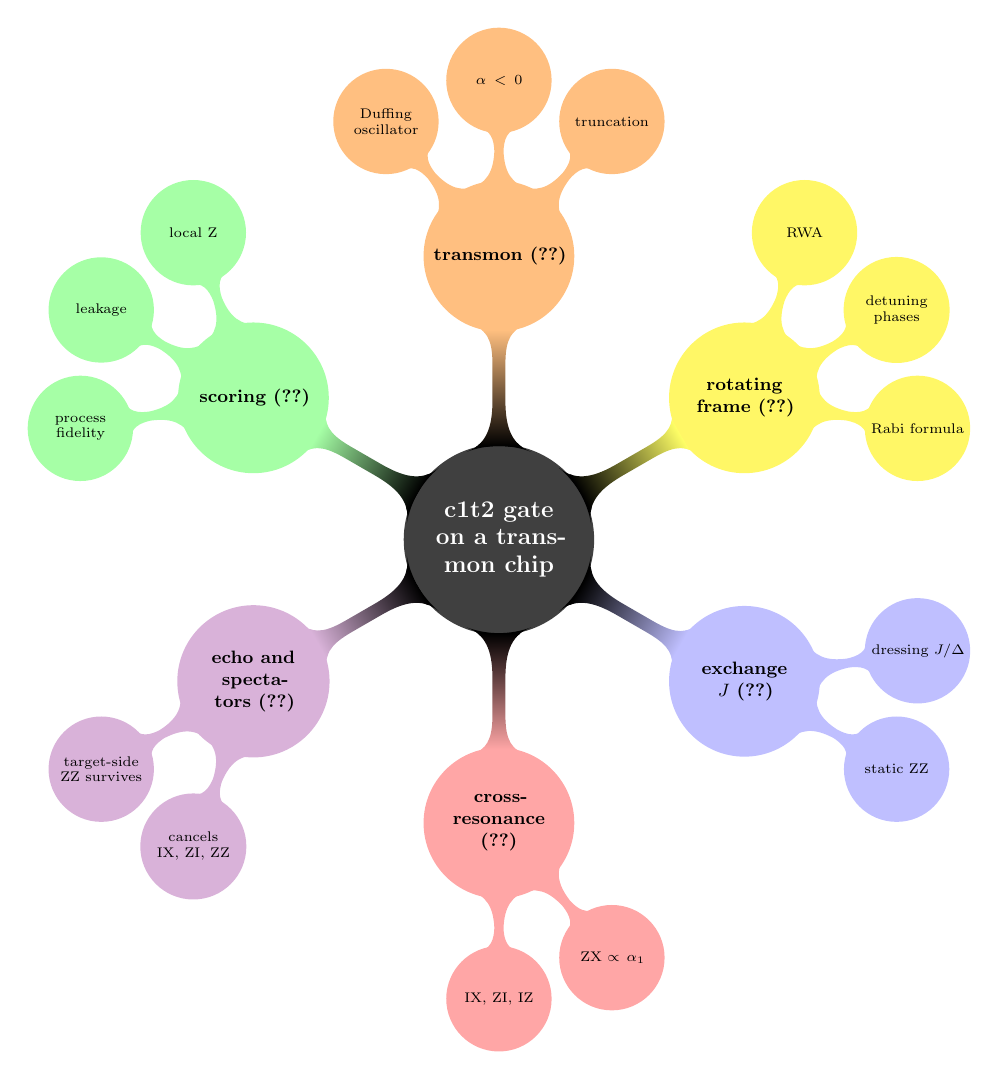
\begin{tikzpicture}[
  mindmap, scale=0.72, transform shape,
  every node/.style={concept, execute at begin node=\hskip0pt},
  root concept/.append style={concept color=black!75, text=white, font=\large\bfseries, minimum size=3.3cm, text width=2.9cm},
  level 1 concept/.append style={level distance=5.0cm, font=\small\bfseries, minimum size=2.6cm, text width=2.3cm},
  level 2 concept/.append style={level distance=3.1cm, sibling angle=40, font=\scriptsize, minimum size=1.8cm, text width=1.65cm},
  text=black
]
\node [root concept] {c1t2 gate on a transmon chip}
  [clockwise from=90, sibling angle=60]
  child [concept color=orange!50] { node {transmon (\cref{sec:transmon})}
    [clockwise from=130]
    child { node {Duffing oscillator} }
    child { node {\(\alpha<0\)} }
    child { node {truncation} } }
  child [concept color=yellow!60] { node {rotating frame (\cref{sec:frames})}
    [clockwise from=70]
    child { node {RWA} }
    child { node {detuning phases} }
    child { node {Rabi formula} } }
  child [concept color=blue!25] { node {exchange \(J\) (\cref{sec:exchange})}
    [clockwise from=10]
    child { node {dressing \(J/\Delta\)} }
    child { node {static ZZ} } }
  child [concept color=red!35] { node {cross-resonance (\cref{sec:cr})}
    [clockwise from=-50]
    child { node {ZX \(\propto \alpha_1\)} }
    child { node {IX, ZI, IZ} } }
  child [concept color=violet!30] { node {echo and spectators (\cref{sec:echo})}
    [clockwise from=-110]
    child { node {cancels IX, ZI, ZZ} }
    child { node {target-side ZZ survives} } }
  child [concept color=green!35] { node {scoring (\cref{sec:fidelity})}
    [clockwise from=-170]
    child { node {process fidelity} }
    child { node {leakage} }
    child { node {local Z} } };
\end{tikzpicture}
\caption{Concept map of Part~\ref{part:physics}. Each first-level node is a section.}
\label{fig:physmap}
\end{figure}

\section{Units and the equation being solved}\label{sec:units}

The code never mentions \(\hbar\) or \(h\). All frequencies are stored in MHz, all times inside the solver are in
\(\mu\)s, and every Hamiltonian coefficient is multiplied by \(2\pi\). So the equation solved is
\[
i\,\frac{d}{dt}\ket{\psi(t)} = H(t)\ket{\psi(t)},\qquad [H] = \text{rad}/\mu\text{s},\quad [t] = \mu\text{s}.
\]
Check: a term \(2\pi f\,\hat n\) with \(f = 1\MHz\) gives a phase of \(2\pi\) on \(\ket{1}\) after \(1\us\), one full
turn. When I write \(H/2\pi\) below, the numbers are frequencies in MHz.

\section{The transmon as a weakly anharmonic oscillator}\label{sec:transmon}

\subsection{From the circuit to the Duffing oscillator}

A transmon is a Josephson junction shunted by a large capacitance. Its Hamiltonian is \cite{koch2007}
\[
H = 4E_C(\hat n - n_g)^2 - E_J\cos\hat\varphi ,
\]
with charging energy \(E_C\), Josephson energy \(E_J\), Cooper-pair number \(\hat n\), and phase \(\hat\varphi\). In the
transmon regime \(E_J/E_C \gtrsim 50\) the dependence on the offset charge \(n_g\) is exponentially small and the phase
stays small, so we expand the cosine:
\[
-E_J\cos\hat\varphi \approx -E_J + \frac{E_J}{2}\hat\varphi^2 - \frac{E_J}{24}\hat\varphi^4 .
\]
The quadratic part is a harmonic oscillator. With
\(\hat\varphi = (2E_C/E_J)^{1/4}(a + \ad)\) and \(\hat n = \tfrac{i}{2}(E_J/2E_C)^{1/4}(\ad - a)\) it becomes
\(\sqrt{8E_JE_C}\,(\ad a + \tfrac12)\). The quartic part is \(-\tfrac{E_C}{12}(a+\ad)^4\). Keeping only the terms that
conserve the number of excitations (the others oscillate at about \(2f\) and \(4f\)),
\((a+\ad)^4 \to 6\,\ad\ad aa + 12\,\ad a + 3\), so
\[
H \approx \big(\sqrt{8E_JE_C} - E_C\big)\,\ad a \;-\; \frac{E_C}{2}\,\ad\ad aa \;+\;\text{const}.
\]
This is a Duffing (Kerr) oscillator with
\[
f_{01} = \sqrt{8E_JE_C} - E_C, \qquad \alpha \equiv f_{12} - f_{01} = -E_C .
\]
So for a transmon the anharmonicity is negative and roughly equal to the charging energy. The code's drift
\cref{eq:drift} is exactly the \(\tfrac{\alpha}{2}\ad\ad aa\) term.

\begin{keybox}[The identity used by the code]
\(\ad\ad aa = \ad(a\ad - 1)a = \hat n^2 - \hat n = \hat n(\hat n-1)\). So in the lab frame the energy of level \(n\) is
\(E_n/h = n f + \tfrac{\alpha}{2}n(n-1)\): \(E_1 = f\), \(E_2 = 2f+\alpha\), \(E_3 = 3f + 3\alpha\). The 1-2 transition is at
\(f+\alpha\). For Q1 that is \(5087.61 - 271.2 = 4816.41\MHz\).
\end{keybox}

\subsection{Truncation}

The code keeps \(N\) levels per qubit: \code{dq.destroy} builds \(N\times N\) matrices with
\(\sqrt{1},\dots,\sqrt{N-1}\) above the diagonal, and anything above level \(N-1\) does not exist. The rule of thumb is to
keep at least one level above anything the dynamics populates, even virtually. The CR interaction goes through the
control's \(\ket{2}\) (\cref{sec:cr}), so Q1 and Q2 have 4 levels; spectators have 3.

\begin{readbox}
\begin{itemize}
\item Koch \emph{et al.} \cite{koch2007}: the original transmon paper. Read the derivation of the energy levels in the
  transmon regime, the result \(\alpha\approx-E_C\), and the exponential suppression of charge dispersion.
\item Krantz \emph{et al.} \cite{krantz2019}, Sec.~II (engineering quantum circuits): harmonic oscillator, the
  transmon, and the Duffing approximation, with figures.
\item Blais \emph{et al.} \cite{blais2021}: the transmon as a Kerr-nonlinear oscillator, in the section on
  superconducting circuits.
\end{itemize}
\end{readbox}

\section{Rotating frames and the rotating-wave approximation}\label{sec:frames}

\subsection{Why rotate}

In the lab frame each qubit's state picks up a phase \(e^{-i2\pi f t}\) with \(f\approx 5\GHz\). That is a phase
turning \(5000\) times per microsecond, which a solver would have to follow. It carries no information about the
gate. So we move to a frame that turns with each qubit and only follow what changes slowly.

\subsection{The transformation}

The lab Hamiltonian of the model is (in MHz, \(H/2\pi\))
\[
\frac{H_{\text{lab}}}{2\pi} = \sum_k\Big[f_k\hat n_k + \frac{\alpha_k}{2}\ad_k\ad_k a_k a_k\Big]
+ \sum_{(i,j)}J_{ij}(a_i+\ad_i)(a_j+\ad_j)
+ \sum_\ell \mathrm{Re}\big[\varepsilon_\ell(t)e^{-i2\pi f^{\text{d}}_\ell t}\big](a_{q_\ell}+\ad_{q_\ell}) .
\eqlab{eq:Hlab}
\]
Define \(U(t) = \exp\big(i\,2\pi t\sum_k f_k\hat n_k\big)\) and \(\ket{\tilde\psi} = U\ket{\psi}\). Then
\(\ket{\tilde\psi}\) obeys the Schr\"odinger equation with
\[
\tilde H = U H U^\dagger + i\,\dot U U^\dagger = U H U^\dagger - 2\pi\sum_k f_k\hat n_k .
\]
The second term cancels the \(f_k\hat n_k\) terms. For the rest we need one identity:
\[
e^{i\theta\hat n}\,a\,e^{-i\theta\hat n} = a\,e^{-i\theta}, \qquad\text{so}\qquad U a_k U^\dagger = a_k e^{-i2\pi f_k t},\quad U\ad_k U^\dagger = \ad_k e^{+i2\pi f_k t}.
\]
Now term by term:
\begin{itemize}
\item The anharmonic term commutes with \(\hat n_k\), so it is unchanged. That is \code{H_drift}.
\item The coupling \(J(a_i+\ad_i)(a_j+\ad_j)\) has four pieces. Two of them,
  \(J\ad_i a_j e^{+i2\pi(f_i-f_j)t}\) and its conjugate, turn at the detuning \(f_i - f_j\approx 100\MHz\). The other two,
  \(J a_i a_j e^{-i2\pi(f_i+f_j)t}\) and its conjugate, turn at about \(10\GHz\). Dropping the fast ones is the
  \emph{rotating-wave approximation} (RWA). What remains is \cref{eq:exch} with \(\Delta_{ij} = f_i - f_j\).
\item The drive \(\tfrac12(\varepsilon e^{-i2\pi f^{\text{d}}t} + \varepsilon^* e^{+i2\pi f^{\text{d}}t})(a e^{-i2\pi f t} + \ad e^{+i2\pi f t})\)
  has slow pieces \(\tfrac12\varepsilon\,\ad e^{-i2\pi(f^{\text{d}}-f)t}\) and its conjugate, and fast pieces at
  \(f^{\text{d}} + f\). Keeping the slow ones gives \cref{eq:drive} with \(\delta = f^{\text{d}} - f\).
\end{itemize}

\begin{keybox}[Why there is no \(f\,\hat n\) term in the code]
The code works in the frame of \cref{eq:Hlab} with each qubit's frame frequency equal to its bare frequency. If you
wanted a frame that differs from the bare frequency, you would need an extra term \(2\pi(f_k - f_k^{\text{frame}})\hat n_k\).
The code has no such term, so \code{frame_MHz} plays both roles. This is gotcha~1 of \cref{sec:gotchas}.
\end{keybox}

\subsection{How good is the RWA here?}

The dropped coupling terms are \(J/(f_i+f_j)\approx 3/10^4\) relative to the kept ones, giving energy shifts of order
\(J^2/(f_i+f_j)\approx 1\kHz\). The dropped drive terms give the Bloch-Siegert shift, of order
\(\Omega^2/(4f)\approx 21^2/(4\cdot 5088)\MHz\approx 22\kHz\) during the CR pulse. Both are small compared to what we
study, but not zero; a full lab-frame simulation would include them.

\subsection{Drives and Rabi oscillations}\label{sec:rabi}

On resonance (\(\delta = 0\)) with constant real \(\varepsilon\), restricted to levels 0 and 1, the drive term is
\(H/2\pi = \tfrac{\varepsilon}{2}\sigma_x\), and the population of \(\ket{1}\) is
\[
P_1(t) = \sin^2(\pi\varepsilon t).
\]
So \(\varepsilon\) in MHz is the Rabi frequency, and a \(\pi\) pulse needs \(\int\varepsilon\,dt = 0.5\MHz\cdot\us\). The Q1
X\(\pi\) has exactly this area (\cref{sec:pulses}).

Off resonance it is convenient to go to the frame of the drive itself. There the two-level Hamiltonian is static:
\[
\frac{H_{\text{d}}}{2\pi} = -\delta\,\ket{1}\!\bra{1} + \frac{\Omega}{2}\big(\ket{0}\!\bra{1} + \ket{1}\!\bra{0}\big),
\eqlab{eq:Hdriveframe}
\]
and starting from \(\ket{0}\) with the drive switched on suddenly one gets Rabi's formula
\[
P_1(t) = \frac{\Omega^2}{\Omega^2+\delta^2}\,\sin^2\!\Big(\pi\sqrt{\Omega^2+\delta^2}\;t\Big).
\eqlab{eq:rabi}
\]
The quantity \(\Omega_R = \sqrt{\Omega^2+\delta^2}\) is the generalized Rabi frequency. Keep \cref{eq:Hdriveframe} in mind:
it is the whole story of the largest micro-oscillation in Part~\ref{part:micro}.

\begin{keybox}[A frame is bookkeeping, but Bloch vectors depend on it]
Populations at the end of a pulse do not depend on the frame. Phases and coherences (Bloch \(X\) and \(Y\)) do: the same
state has \(X, Y\) turning at \(|\delta|\) in one frame and standing still in another. Every Bloch plot in this project is
drawn in the frame of \code{frame_MHz}.
\end{keybox}

\begin{readbox}
\begin{itemize}
\item Sakurai and Napolitano \cite{sakurai}, Sec.~5.5 (time-dependent potentials and the interaction picture,
  including the time-dependent two-state problem and Rabi's formula).
\item Steck \cite{steck}, Ch.~5: rotating frame, rotating-wave approximation, Rabi flopping on and off resonance.
  Free online and very clear.
\item Krantz \emph{et al.} \cite{krantz2019}, Sec.~IV (qubit control): the drive Hamiltonian of a transmon, the
  rotating frame, and single-qubit gates.
\end{itemize}
\end{readbox}

\section{Exchange coupling, dressing, and static ZZ}\label{sec:exchange}

\subsection{Where \texorpdfstring{\(J\)}{J} comes from}

Two transmons coupled through a capacitor have an interaction proportional to \(\hat n_1\hat n_2\). Since
\(\hat n\propto i(\ad - a)\), this is \(-g(\ad_1 - a_1)(\ad_2 - a_2)\), and after the RWA only
\(J(\ad_1 a_2 + a_1\ad_2)\) survives \cite{krantz2019,blais2021}. The code stores \(J\) directly.

\subsection{Dressing}

Look at the single-excitation states \(\ket{10}\) and \(\ket{01}\) of two qubits. In the lab frame
\[
\frac{H}{2\pi} = \begin{pmatrix} f_1 & J\\ J & f_2\end{pmatrix},\qquad
E_\pm = \frac{f_1+f_2}{2} \pm \sqrt{\frac{\Delta^2}{4}+J^2},\qquad \Delta = f_1-f_2 .
\]
For \(|J|\ll|\Delta|\) the eigenstates are \(\ket{10} + \tfrac{J}{\Delta}\ket{01}\) and
\(\ket{01} - \tfrac{J}{\Delta}\ket{10}\) (to first order), and the levels move apart by \(J^2/\Delta\) each. So:

\begin{keybox}[Two numbers to remember]
\emph{Hybridization amplitude} \(J/\Delta\): how much of the neighbour's excitation each dressed state contains.
\emph{Dressed shift} \(J^2/\Delta\): how far each qubit's frequency moves. For Q3 on Q2:
\(J/\Delta = 3.546/109.59 = 0.0324\) and \(J^2/\Delta = 114.7\kHz\) (Q2 down, Q3 up).
\end{keybox}

\subsection{Static ZZ}

The four computational energies of two coupled transmons are not additive. Define
\[
\zeta = E_{11} - E_{10} - E_{01} + E_{00}.
\]
Second-order perturbation theory gives the shifts. \(\ket{10}\) and \(\ket{01}\) push each other by \(\pm J^2/\Delta\),
which cancels in \(\zeta\). \(\ket{11}\) couples to \(\ket{20}\) and \(\ket{02}\) with matrix element \(\sqrt2 J\), at energy
differences \(E_{11}-E_{20} = -(\Delta + \alpha_1)\) and \(E_{11}-E_{02} = \Delta - \alpha_2\). So
\[
\zeta \approx \frac{2J^2}{\Delta-\alpha_2} - \frac{2J^2}{\Delta+\alpha_1}
= \frac{2J^2(\alpha_1+\alpha_2)}{(\Delta+\alpha_1)(\Delta-\alpha_2)} . \eqlab{eq:zz}
\]
The \(\ket{2}\) levels are the whole reason ZZ exists: for two-level qubits \(\zeta = 0\).

\begin{table}[htbp]
\centering\small
\caption{Static ZZ: formula \cref{eq:zz} against exact diagonalization (5 levels per qubit).}
\label{tab:zz}
\begin{tabular}{@{}l c c c c c@{}}
\toprule
edge & \(J\) (MHz) & \(\Delta\) (MHz) & \(\alpha_i,\ \alpha_j\) (MHz) & formula (kHz) & exact (kHz) \\
\midrule
c1\_t2 & 3.2163 & \(+104.15\) & \(-271.2,\ -266.4\) & 179.69 & 179.53 \\
c3\_t2 & 3.5456 & \(+109.59\) & \(-268.0,\ -266.4\) & 225.59 & 225.32 \\
c1\_t2 with \(\alpha_2 = +266.4\) & 3.2163 & \(+104.15\) & \(-271.2,\ +266.4\) & \(-3.66\) & \(-3.66\) \\
\bottomrule
\end{tabular}
\end{table}

\begin{figure}[htbp]
\centering
\includegraphics[width=0.85\textwidth]{figures/zz_vs_detuning.pdf}
\caption{Static ZZ against detuning. Blue: two transmons. Green: the same pair with the sign of \(\alpha_2\) flipped. The
numerator \(\alpha_1+\alpha_2\) nearly vanishes, so ZZ is suppressed by a factor of about 50 at the c1\_t2 detuning. This
is the physics behind opposite-sign-anharmonicity couplers \cite{ku2020,zhao2020}, and it is why flipping the sign of
\(\alpha_2,\alpha_3\) changed the Q2 and Q3 curves in the earlier plots. Spikes are where levels cross and labels swap.}
\label{fig:zz}
\end{figure}

\begin{warnbox}[A sign typo in PAPER\_VALUES.md]
\code{PAPER_VALUES.md} writes the denominator as \((\Delta+\alpha_1)(\alpha_2-\Delta)\). That has the opposite sign
from \cref{eq:zz}; the magnitude is right. The code does not use the formula (it diagonalizes exactly), so no number
is affected.
\end{warnbox}

On the Q1 Q2 Q3 chip with both edges on, exact diagonalization gives \(\zeta_{12} = 181.1\kHz\),
\(\zeta_{23} = 223.5\kHz\), and \(\zeta_{13} = 0.36\kHz\) (Q1 and Q3 are not directly coupled). Q2's dressed frequency moves
by \(-114.4\kHz\) and Q3's by \(+116.6\kHz\) when c3\_t2 is switched on.

\begin{readbox}
\begin{itemize}
\item Krantz \emph{et al.} \cite{krantz2019}, Sec.~IV: capacitive coupling of two transmons and the exchange
  Hamiltonian.
\item Blais \emph{et al.} \cite{blais2021}: dispersive and Schrieffer-Wolff treatment of coupled modes, which is
  exactly the dressing above.
\item Bravyi, DiVincenzo, Loss \cite{bravyi2011}: the general theory of the Schrieffer-Wolff transformation, if you
  want to know why second-order perturbation theory gives effective Hamiltonians.
\item Ku \emph{et al.} \cite{ku2020} and Zhao \emph{et al.} \cite{zhao2020}: the static ZZ formula and how
  opposite-sign anharmonicity cancels it.
\end{itemize}
\end{readbox}

\section{Cross-resonance}\label{sec:cr}

\subsection{The idea}

Drive the control (Q1) at the target's frequency \(f_2\). The control itself is far off resonance and only wiggles
(that wiggle is the main micro-oscillation of Part~\ref{part:micro}). Through \(J\) a small part of the drive leaks to
the target, where it is resonant, and the size of the leak depends on the control's state. A target drive whose
amplitude depends on the control is a ZX interaction \cite{rigetti2010,chow2011}.

\subsection{A derivation you can check by hand}

Work in a frame where both qubits rotate at the drive frequency \(f_2\). Then (levels \(\ket{n_1 n_2}\), energies in MHz)
\(E_{00} = 0\), \(E_{01} = 0\), \(E_{10} = \Delta\), \(E_{11} = \Delta\), \(E_{20} = 2\Delta + \alpha_1\), with
\(\Delta = f_1 - f_2 = 104.15\MHz\). The drive \(\tfrac{\Omega}{2}(a_1+\ad_1)\) connects states that differ by one
control quantum; the exchange \(J(\ad_1a_2+a_1\ad_2)\) swaps one quantum between the qubits (\cref{fig:crlevels}).

\begin{figure}[htbp]
\centering
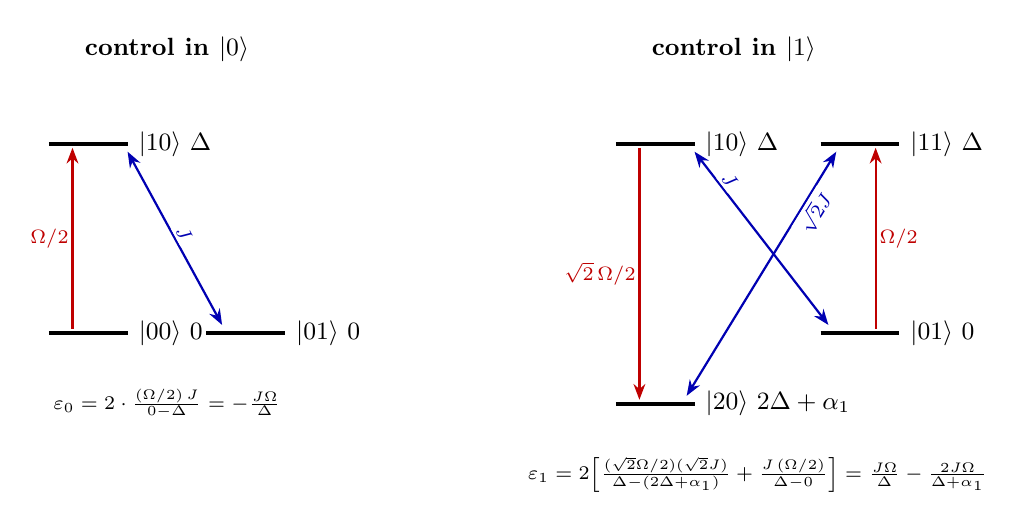
\begin{tikzpicture}[x=1cm,y=1cm,
  lev/.style={line width=1.4pt},
  st/.style={font=\small},
  dr/.style={-{Stealth[length=2mm]}, red!75!black, thick},
  ex/.style={{Stealth[length=2mm]}-{Stealth[length=2mm]}, blue!70!black, thick},
  lab/.style={font=\scriptsize, fill=white, inner sep=1pt}]
% control in 0 panel
\begin{scope}
\node[font=\small\bfseries] at (1.5,3.6) {control in \(\ket{0}\)};
\draw[lev] (0,0) -- (1,0) node[st, right] {\(\ket{00}\)\ \(0\)};
\draw[lev] (2,0) -- (3,0) node[st, right] {\(\ket{01}\)\ \(0\)};
\draw[lev] (0,2.4) -- (1,2.4) node[st, right] {\(\ket{10}\)\ \(\Delta\)};
\draw[dr] (0.3,0.05) -- node[lab, left] {\(\Omega/2\)} (0.3,2.35);
\draw[ex] (1.0,2.3) -- node[lab, sloped, above] {\(J\)} (2.2,0.1);
\node[font=\scriptsize, align=center] at (1.5,-0.9) {\(\varepsilon_0 = 2\cdot\frac{(\Omega/2)\,J}{0-\Delta} = -\frac{J\Omega}{\Delta}\)};
\end{scope}
% control in 1 panel
\begin{scope}[xshift=7.2cm]
\node[font=\small\bfseries] at (1.5,3.6) {control in \(\ket{1}\)};
\draw[lev] (0,2.4) -- (1,2.4) node[st, right] {\(\ket{10}\)\ \(\Delta\)};
\draw[lev] (2.6,2.4) -- (3.6,2.4) node[st, right] {\(\ket{11}\)\ \(\Delta\)};
\draw[lev] (0,-0.9) -- (1,-0.9) node[st, right] {\(\ket{20}\)\ \(2\Delta+\alpha_1\)};
\draw[lev] (2.6,0) -- (3.6,0) node[st, right] {\(\ket{01}\)\ \(0\)};
\draw[dr] (0.3,2.35) -- node[lab, left] {\(\sqrt2\,\Omega/2\)} (0.3,-0.85);
\draw[ex] (0.9,-0.8) -- node[lab, sloped, below, pos=0.78] {\(\sqrt2 J\)} (2.8,2.3);
\draw[ex] (1.0,2.3) -- node[lab, sloped, above, pos=0.2] {\(J\)} (2.7,0.1);
\draw[dr] (3.3,0.05) -- node[lab, right] {\(\Omega/2\)} (3.3,2.35);
\node[font=\scriptsize, align=center] at (1.8,-1.8) {\(\varepsilon_1 = 2\Big[\frac{(\sqrt2\Omega/2)(\sqrt2J)}{\Delta-(2\Delta+\alpha_1)} + \frac{J\,(\Omega/2)}{\Delta-0}\Big] = \frac{J\Omega}{\Delta} - \frac{2J\Omega}{\Delta+\alpha_1}\)};
\end{scope}
\end{tikzpicture}
\caption{Second-order paths that move the target from 0 to 1. Red: CR drive on the control. Blue: exchange. Energies are
in the frame of the drive (both qubits rotating at \(f_2\)). With the control in \(\ket{1}\) there is a path through the
control's \(\ket{2}\), which is why the result depends on \(\alpha_1\).}
\label{fig:crlevels}
\end{figure}

Second-order perturbation theory gives the effective coupling between two degenerate states \(i\) and \(f\) as
\(\sum_m V_{fm}V_{mi}/(E_i - E_m)\). Doing this for both control states (\cref{fig:crlevels}) gives an effective target drive
\(\tfrac{\varepsilon_c}{2}(a_2+\ad_2)\) whose amplitude \(\varepsilon_c\) depends on the control state \(c\). Writing
\(\ket{0}\!\bra{0} = \tfrac12(I+Z)\) and \(\ket{1}\!\bra{1} = \tfrac12(I-Z)\),
\[
\begin{gathered}
\frac{H_{\text{eff}}}{2\pi} = \frac{\nu_{IX}}{2}\,I\!X + \frac{\nu_{ZX}}{2}\,Z\!X + \dots,\\[0.5em]
\nu_{ZX} = \frac{\varepsilon_0-\varepsilon_1}{2} = -\frac{J\Omega}{\Delta}\,\frac{\alpha_1}{\Delta+\alpha_1},\qquad
\nu_{IX} = \frac{\varepsilon_0+\varepsilon_1}{2} = -\frac{J\Omega}{\Delta+\alpha_1}.
\end{gathered}
\eqlab{eq:zx}
\]
The same leading-order expression appears, with each paper's own sign and factor conventions, in
\cite{magesan2020,tripathi2019,malekakhlagh2020}.

\begin{table}[htbp]
\centering\small
\caption{Leading-order CR rates for c1t2 (\(J = 3.216\MHz\), \(\Omega = 21\MHz\), \(\Delta = 104.15\MHz\)).}
\label{tab:cr}
\begin{tabular}{@{}l c c c@{}}
\toprule
control anharmonicity & \(\nu_{ZX}\) (MHz) & \(\nu_{IX}\) (MHz) & time for ZX(\(\pi/2\)), \(1/(4|\nu_{ZX}|)\) \\
\midrule
\(\alpha_1 = -271.2\MHz\) (transmon) & \(-1.053\) & \(+0.404\) & 237~ns \\
\(\alpha_1 = +271.2\MHz\) (wrong sign) & \(-0.469\) & \(-0.180\) & 534~ns \\
\bottomrule
\end{tabular}
\end{table}

Three checks against the code. (i) The sign: \(\nu_{ZX}<0\) with positive \(\Omega\), so the gate rotates as
\(\exp(+i\tfrac{\theta}{2}Z\!X)\), which is ZX(\(-\pi/2\)), the \code{zx_m90} target. (ii) The size: the pulse has a
flat-equivalent CR time of \(2\times(122 + 2\times 6.29) = 269\ns\), against 237~ns from \cref{eq:zx}. The 13\%
difference is expected: at \(\Omega/\Delta\approx0.2\) higher-order terms reduce \(\nu_{ZX}\) \cite{magesan2020}. (iii) The
anharmonicity: the CR rate depends on the \emph{control's} \(\alpha_1\), through the \(\ket{2}\) path; flipping its sign
slows the gate by a factor of 2.2. The sign of the target and spectator anharmonicities enters through ZZ instead
(\cref{fig:zz}).

\subsection{The other terms}

A full treatment \cite{sheldon2016,magesan2020} gives terms \(I\!X\), \(I\!Y\), \(I\!Z\), \(Z\!I\), \(Z\!X\), \(Z\!Y\), \(Z\!Z\).
\(Z\!I\) is the AC Stark shift of the control by its own off-resonant drive: the dressed 0-1 splitting of Q1 in the drive
frame becomes 107.5~MHz instead of 104.15~MHz (\cref{sec:micro-drive}). \(Z\!Z\) has a static part (\cref{eq:zz}) and a
drive-induced part. In this model there is no classical crosstalk (the CR line touches only Q1), so \(I\!X\) comes only
through \(J\).

\begin{readbox}
In this order:
\begin{enumerate}
\item Rigetti and Devoret \cite{rigetti2010}: where the CR idea for superconducting qubits starts.
\item Chow \emph{et al.} \cite{chow2011}: the first demonstration, short and readable.
\item Sheldon \emph{et al.} \cite{sheldon2016}: CR Hamiltonian tomography, all the terms above, and how to tune the echo.
\item Magesan and Gambetta \cite{magesan2020}: the effective Hamiltonian, derived carefully, including higher orders.
\item Tripathi \emph{et al.} \cite{tripathi2019} and Malekakhlagh \emph{et al.} \cite{malekakhlagh2020}: error
  budgets and first-principles analysis, for when you want every term.
\end{enumerate}
\end{readbox}

\section{The echo, and why spectators on the two sides differ}\label{sec:echo}

\subsection{What the echo cancels}

The sequence is CR(\(+\)), X\(\pi\) on the control, CR(\(-\)), X\(\pi\). Two rules decide the fate of each term:
\begin{itemize}
\item CR(\(-\)) flips the sign of every term \emph{odd} in \(\Omega\) (\(I\!X, I\!Y, Z\!X, Z\!Y\)).
\item Conjugating by X on the control flips every term with a \(Z\) on the control (\(Z\!I, Z\!X, Z\!Y, Z\!Z\)), since
  \(XZX = -Z\).
\end{itemize}
The second half contributes each term with the product of both signs. Adding it to the first half:

\begin{center}\small
\begin{tabular}{@{}l c c c c@{}}
\toprule
term & odd in \(\Omega\)? & \(Z\) on control? & sign in second half & net \\
\midrule
\(Z\!X\), \(Z\!Y\) & yes & yes & \((-)(-) = +\) & \textbf{kept} (doubled) \\
\(I\!X\), \(I\!Y\) & yes & no & \((-)(+) = -\) & cancelled \\
\(Z\!I\) & no & yes & \((+)(-) = -\) & cancelled \\
\(Z\!Z\) (control-target) & no & yes & \((+)(-) = -\) & cancelled \\
\(I\!Z\) & no & no & \(+\) & kept \\
\bottomrule
\end{tabular}
\end{center}

This is first order (it ignores that the terms do not commute) but it is the reason the echo is used
\cite{corcoles2013,sheldon2016}.

\subsection{Spectators}\label{sec:spectators}

Apply the same rules to a spectator \(s\):
\begin{itemize}
\item \emph{Control-side spectator} (Q4 or Q6 coupled to Q1): the ZZ term is \(Z_1Z_s\). It has a \(Z\) on the control,
  so the echo cancels it. That is why Q4 barely hurt the gate in Phase 3 (Q6 hurt for a different reason: it sits
  2.2~MHz from the CR tone and gets driven).
\item \emph{Target-side spectator} (Q3 coupled to Q2): the ZZ term is \(Z_2Z_3\). The echo acts on Q1 only, so it
  is \emph{not} cancelled. Worse, the CR rotates Q2 about \(X\), which does not commute with \(Z_2Z_3\), so Q3's phase
  becomes entangled with where Q2 is on its Bloch sphere.
\end{itemize}
This is the main subject of Sundaresan \emph{et al.} \cite{sundaresan2020}.

\subsection{What this means for the Q1 Q2 Q3 numbers}

\begin{center}\small
\begin{tabular}{@{}l c c l@{}}
\toprule
case & \(F_{\text{pro}}\) & Q3 left its state & main cause \\
\midrule
2Q simulator, no filter & 0.991747 & & reference \\
Q1 Q2 Q3, c3\_t2 off & 0.991747 & 0 & identical to 2Q \\
c3\_t2 on, Q3 in \(\ket{0}\) & 0.968690 & 0.5\% & Q2 dressed shift \(-114\kHz\), uncompensated \\
c3\_t2 on, Q3 in \(\ket{1}\) & 0.971776 & 0.7\% & shift \(-114 + 223 = +109\kHz\) \\
c3\_t2 on, Q3 in \(\ket{+}\) & 0.887044 & 9.9\% & the two shifts at once: ZZ entangles Q2 and Q3 \\
\bottomrule
\end{tabular}
\end{center}

Two back-of-the-envelope checks. For Q3 in \(\ket{0}\), a Z rotation of Q2 by
\(\phi = 2\pi\times0.1144\MHz\times0.412\us = 0.30\) rad reduces the process fidelity by \(\cos^2(\phi/2) = 0.978\), and
\(0.9917\times0.978 = 0.970\), close to 0.9687. This part is a local Z error that frame compensation or a virtual Z
would remove. For Q3 in \(\ket{+}\), the phase difference between the two Q3 branches is
\(2\pi\times\zeta_{23}\times T = 2\pi\times0.2235\times0.412 = 0.58\) rad, close to the 0.59~rad measured; this part is
entangling and cannot be removed by local frame updates. With the lab Q3 frequency (5018.15~MHz, only 34.7~MHz above
Q2) both effects grow, and the process fidelities drop to 0.898 (Q3 in \(\ket{0}\)), 0.961 (Q3 in \(\ket{1}\)) and
0.784 (Q3 in \(\ket{+}\)).

\begin{readbox}
Sundaresan \emph{et al.} \cite{sundaresan2020}: spectator errors in CR gates and how rotary echoes on the target
suppress them. C\'orcoles \emph{et al.} \cite{corcoles2013}: the echoed CR. Sheldon \emph{et al.} \cite{sheldon2016}:
echo tuning.
\end{readbox}

\section{How a gate is scored}\label{sec:fidelity}

With the \(4\times4\) block \(M\) (rows: final computational states, columns: initial ones) and target \(U_t\) (here
ZX(\(-\pi/2\))):
\[
F_{\text{pro}} = \frac{|\Tr(U_t^\dagger M)|^2}{d^2},\qquad
F_{\text{avg}} = \frac{|\Tr(U_t^\dagger M)|^2 + d}{d(d+1)},\qquad
L = \frac1d\sum_c\Big(1-\sum_r |M_{rc}|^2\Big),\qquad d = 4 .
\]

\src{../two_qubit_simulator/optimization/fidelity.py}{100}{134}

The global phase drops out of \(|\Tr|^2\). \emph{Local Z rotations do not}: a Z rotation of either qubit after the gate
lowers \(F_{\text{pro}}\). In hardware such rotations are often removed for free by shifting the phase of later pulses
(virtual Z, \cite{mckay2017}); here nothing removes them. For a unitary block
\(F_{\text{avg}} = (dF_{\text{pro}}+1)/(d+1)\) \cite{nielsen2002}; with leakage use the corrected formula of
\cite{pedersen2007}, and see \cite{wood2018} for what leakage does to benchmarking.

\begin{readbox}
Nielsen \cite{nielsen2002} (average fidelity from process fidelity), Pedersen, M\o ller, M\o lmer \cite{pedersen2007}
(fidelity with leakage), Wood and Gambetta \cite{wood2018} (leakage), McKay \emph{et al.} \cite{mckay2017} (virtual Z).
\end{readbox}

\section{How the solver works}\label{sec:solver}

\code{dq.sesolve} integrates the linear ODE \(\dot\psi = -iH(t)\psi\). It uses Tsit5, an explicit Runge-Kutta method of
order 5 with an embedded order-4 solution \cite{tsitouras2011}. At each step the difference between the two solutions
estimates the error; if the error exceeds \(\text{atol} + \text{rtol}\times|\psi|\) the step is rejected and shrunk,
otherwise it is accepted and the next step size is chosen from the error \cite{hairer1993}. Two settings matter:
\begin{itemize}
\item \textbf{\code{discontinuity_ts}}: the envelopes jump every nanosecond. Runge-Kutta methods assume a smooth
  right-hand side; stepping across a jump wastes steps or loses accuracy. Listing the jump times makes the solver end
  a step exactly at each jump and restart.
\item \textbf{Tolerance}: \(10^{-10}\) by default, \(10^{-12}\) in \code{C1T2FlatFidelity}. Our effects are \(10^{-3}\) and
  larger, so numerical error is not a candidate explanation for anything in the plots.
\end{itemize}
dynamiqs \cite{dynamiqs} builds on JAX \cite{jax} and uses the Diffrax ODE library \cite{kidger2021}. JAX compiles the
right-hand side and can batch over initial states, which is what \code{run_shot_batch} uses (versions here: dynamiqs
0.3.4, JAX 0.6.2, Diffrax 0.7.2).

\begin{readbox}
Hairer, N\o rsett, Wanner \cite{hairer1993}, Sec.~II.4 (error estimation and step-size selection). Tsitouras
\cite{tsitouras2011} (the Tsit5 coefficients). Kidger \cite{kidger2021} (Diffrax, Ch.~on numerical solvers).
\end{readbox}

%=====================================================================
\part{The micro-oscillations}\label{part:micro}
%=====================================================================

\section{What you see}\label{sec:micro-what}

\begin{figure}[htbp]
\centering
\includegraphics[width=0.92\textwidth]{../figures/c1t2_flat_xyz_q3_ground.png}
\caption{The plot that started the question: Bloch components of Q1, Q2, Q3 through the echoed c1t2 flat-top, c3\_t2
on, Q2 and Q3 starting in \(\ket{0}\), sampled every 2~ns.}
\label{fig:original}
\end{figure}

There are four distinct features:
\begin{enumerate}[label=\textbf{\Alph*.}]
\item Q1's \(X\) and \(Y\) oscillate fast, with amplitude about 0.2, whenever the CR tone is on.
\item Q1's \(Z\) sits near \(\pm0.98\) instead of \(\pm1\) during the CR, with small wiggles.
\item Q3's \(X\) and \(Y\) show small fast ripples once Q2 has moved away from \(\ket{0}\).
\item Q2 shows small kinks during the two X\(\pi\) echo pulses.
\end{enumerate}

\begin{keybox}[The short answer]
None of them is noise or numerical error (the solver tolerance is \(10^{-12}\)). All four are the same phenomenon:
\textbf{the true eigenstates of the driven, coupled chip are not the bare states, and the plot shows the state in the
bare rotating frame.} A state that sits still in its own (dressed) frame looks like it is turning when seen from a
frame that rotates at a different rate. A and B come from dressing by the CR drive; C and D come from dressing by the
always-on exchange couplings.
\end{keybox}

The irregular envelope of the fast oscillations in \cref{fig:original} is a plotting artifact: a 9.6~ns period sampled
every 2~ns has only 4.8 points per period. The figures below sample every 0.25~ns.

\section{A: the CR tone dresses Q1}\label{sec:micro-drive}

\subsection{The model}

For Q1 the CR tone is an off-resonant drive with \(\Omega = 21\MHz\) and \(\delta = f_2 - f_1 = -104.15\MHz\). In the
frame of the drive the two-level Hamiltonian is the static \cref{eq:Hdriveframe}. Its eigenstates are tilted away
from \(\ket{0}\) and \(\ket{1}\). The one connected to \(\ket{0}\) is
\[
\ket{\tilde0} = \cos\tfrac{\theta}{2}\ket{0} - \sin\tfrac{\theta}{2}\ket{1},\qquad \tan\theta = \frac{\Omega}{|\delta|},
\]
with Bloch vector \((X,Y,Z) = (-\sin\theta,\,0,\,\cos\theta)\). Numbers: \(\theta = 0.199\) rad (11.4 degrees),
\(\sin\theta = 0.198\), \(\cos\theta = 0.980\).

If the drive is switched on slowly compared with \(1/\Omega_R\) (adiabatically), the state follows \(\ket{\tilde0}\): in
the drive frame the Bloch vector simply tilts by \(\theta\) and stays there.

\subsection{Back to the qubit frame}

The simulator's frame turns at \(f_1\), not at \(f_2\). Going from the drive frame to the qubit frame multiplies the
\(\ket{1}\) amplitude by \(e^{-i2\pi\delta t}\), so \(\rho_{01}\to\rho_{01}e^{+i2\pi\delta t}\) and
\[
\big(X(t),\,Y(t)\big) = \sin\theta\,\big(-\cos 2\pi\delta t,\ \sin 2\pi\delta t\big),\qquad Z = \cos\theta .
\eqlab{eq:circle}
\]
The tilted vector turns about \(z\) at \(|\delta| = 104.15\MHz\) (period 9.60~ns) with radius \(\sin\theta\approx0.2\).
That is feature A. \(Z\) stays at \(\cos\theta = 0.98\). That is the offset in feature B.

\begin{figure}[htbp]
\centering
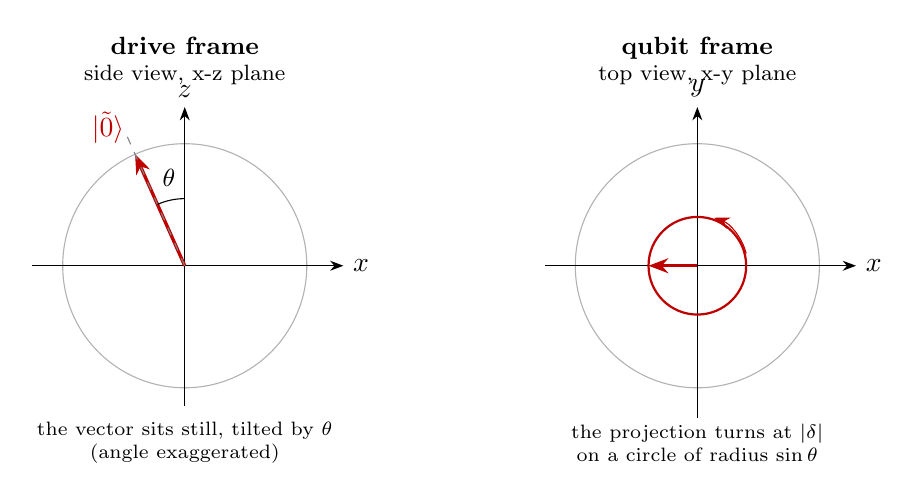
\begin{tikzpicture}[scale=1.55]
\begin{scope}
\node[font=\small\bfseries, align=center] at (0,1.68) {drive frame\\[-0.15em]{\mdseries\footnotesize side view, x-z plane}};
\draw[gray!60] (0,0) circle (1);
\draw[-{Stealth}] (-1.25,0) -- (1.3,0) node[right] {\(x\)};
\draw[-{Stealth}] (0,-1.15) -- (0,1.3) node[above] {\(z\)};
\draw[-{Stealth[length=2.5mm]}, very thick, red!75!black] (0,0) -- ({-sin(24)},{cos(24)}) node[above left] {\(\ket{\tilde 0}\)};
\draw[dashed, gray] (0,0) -- ({-1.2*sin(24)},{1.2*cos(24)});
\draw (0,0.55) arc (90:114:0.55);
\node[font=\small] at (-0.13,0.72) {\(\theta\)};
\node[font=\scriptsize, align=center] at (0,-1.45) {the vector sits still, tilted by \(\theta\)\\ (angle exaggerated)};
\end{scope}
\begin{scope}[xshift=4.2cm]
\node[font=\small\bfseries, align=center] at (0,1.68) {qubit frame\\[-0.15em]{\mdseries\footnotesize top view, x-y plane}};
\draw[gray!60] (0,0) circle (1);
\draw[-{Stealth}] (-1.25,0) -- (1.3,0) node[right] {\(x\)};
\draw[-{Stealth}] (0,-1.25) -- (0,1.3) node[above] {\(y\)};
\draw[thick, red!75!black] (0,0) circle (0.4);
\draw[-{Stealth[length=2.5mm]}, very thick, red!75!black] (0,0) -- (-0.4,0);
\draw[-{Stealth[length=2mm]}, red!75!black] (0.4,0.1) arc (14:70:0.42);
\node[font=\scriptsize, align=center] at (0,-1.45) {the projection turns at \(|\delta|\)\\ on a circle of radius \(\sin\theta\)};
\end{scope}
\end{tikzpicture}
\caption{The same dressed state seen from two frames. Left: in the frame of the CR tone, Q1's Bloch vector stands
still, tilted by \(\theta\) toward \(-x\). Right: in Q1's own frame (the simulator's), that tilted vector precesses about
\(z\) at the detuning, so \(X\) and \(Y\) oscillate with amplitude \(\sin\theta\).}
\label{fig:blochsketch}
\end{figure}

\subsection{The evidence}

\begin{figure}[htbp]
\centering
\includegraphics[width=0.98\textwidth]{figures/micro_q1_frames.pdf}
\caption{Q1 during CR(\(+\)), from the full Q1 Q2 Q3 simulation. Left: the simulator's frame, \(X\) and \(Y\) turn at
104~MHz inside the dotted envelope \(\pm\)(dressed-state amplitude). Right: the same states in the frame of the CR tone:
the fast oscillation is gone and the vector sits on the dressed eigenstate (dashed), up to a small residual wiggle
(feature B, next section).}
\label{fig:q1frames}
\end{figure}

\begin{itemize}
\item \textbf{Amplitude.} Simulation: \(2|\rho_{01}| = 0.1920\) (Q1 from \(\ket{0}\)) and 0.1930 (from \(\ket{1}\)). Dressed
  eigenstates of the 4-level Q1: 0.1912 and 0.1938. Two-level formula: \(\sin\theta = 0.1977\). The small difference is
  Q1's \(\ket{2}\) level.
\item \textbf{Frequency.} The spectrum of Q1's coherence over a 2~\(\mu\)s CR tone peaks at \(-104.13\MHz\); prediction
  \(f_2 - f_1 = -104.15\MHz\) (\cref{fig:spectrum}, top).
\item \textbf{Scaling.} Changing \(\Omega\) and \(\delta\) moves the amplitude exactly as the dressed-state formula says
  (\cref{fig:scan}); the largest deviation over the whole scan is 0.034, at points where the 16~ns ramp is least
  adiabatic.
\end{itemize}

\begin{figure}[htbp]
\centering
\includegraphics[width=0.98\textwidth]{figures/micro_amplitude_scan.pdf}
\caption{Oscillation amplitude of a lone Q1 (couplings off) under a 21~MHz-style flat-top CR tone. Left: against drive
strength at the c1t2 detuning. Right: against detuning at 21~MHz. Points are simulations, solid lines the dressed
eigenstates of a 4-level transmon, dotted the two-level \(\sin\theta\). Two resonances of the transmon are marked: the
1-2 transition at \(\delta=\alpha_1\), and the two-photon 0-2 transition at \(\delta=\alpha_1/2 = -135.6\MHz\), only
31~MHz from where the c1t2 CR tone sits. The latter is one of the standard frequency-collision conditions for CR
\cite{hertzberg2021}.}
\label{fig:scan}
\end{figure}

\section{B: the ramp is not perfectly adiabatic}\label{sec:micro-ramp}

Adiabatic following needs the tilt angle to change slowly compared with the dressed splitting:
\(|\dot\theta|\ll 2\pi\Omega_R\). For the 16~ns ramp, \(\theta\) goes from 0 to 0.199 rad, so on average
\(\dot\theta\approx0.012\) rad/ns, against \(2\pi\Omega_R = 2\pi\times106\MHz = 0.67\) rad/ns. That is a ratio of about
0.02: mostly adiabatic, but not perfectly. The ramp also meets the flat top with a kink (its slope drops from about
1.5~MHz/ns to zero within two samples). Whatever is not followed adiabatically appears as a small nutation of the
Bloch vector about the tilted axis, at the dressed splitting.

\begin{figure}[htbp]
\centering
\includegraphics[width=0.98\textwidth]{figures/micro_ramp.pdf}
\caption{Lone Q1, CR tone 21~MHz, couplings off. Orange: square turn-on; the vector nutates about the tilted axis with
cone angle \(\theta\), so \(Z\) swings between 1 and \(\cos2\theta = 0.922\) (simulated minimum 0.925) and the drive-frame
\(X\) swings by \(\sin2\theta = 0.388\) (simulated 0.385). It also does not return to \(Z=1\) when the pulse stops
abruptly. Blue: the real 16~ns ramp; the residual swings are 0.011 in \(Z\) and 0.057 in \(X\), seven times smaller, and
\(Z\) returns to 1.000 after the ramp down.}
\label{fig:ramp}
\end{figure}

The wiggles of \(Z\) sit at the dressed splitting. In the drive frame, the 4-level Q1 has its \(\ket{\tilde0}\) at
\(-1.01\MHz\) and \(\ket{\tilde1}\) at \(106.49\MHz\), a splitting of 107.5~MHz (two-level value: \(\Omega_R = 106.25\MHz\); bare:
104.15~MHz; the 3.4~MHz difference is the AC Stark shift, the \(Z\!I\) term of \cref{sec:cr}). The spectrum of \(Z\) in
\cref{fig:spectrum} has its strongest line there. The much weaker lines near \(\pm63\) and \(\pm170\MHz\) are beats with the
dressed \(\ket{\tilde2}\) state, which the ramp also populates very slightly.

\begin{figure}[htbp]
\centering
\includegraphics[width=0.92\textwidth]{figures/micro_spectrum.pdf}
\caption{A 2~\(\mu\)s flat CR tone on the full Q1 Q2 Q3 chip, starting in \(\ket{000}\). Spectra of each qubit's 0-1
coherence in its own frame, and of Q1's \(Z\). Dashed lines are predictions with no fitting: Q1 at \(f_2-f_1\), Q1's \(Z\)
at the 4-level dressed splitting, Q3 at \(f_2-f_3\). The peak near 0 is the slow, intended dynamics (for Q2, the CR
rotation itself). Q2's own fast lines are below \(10^{-3}\): it starts in \(\ket{0}\), so its partners' coherences reach it
only at second order.}
\label{fig:spectrum}
\end{figure}

\section{C: exchange dressing makes Q3 ripple}\label{sec:micro-exchange}

Q3 is never driven. But it is coupled to Q2 by \(J = 3.546\MHz\) at a detuning \(\Delta_{32} = f_3 - f_2 = 109.59\MHz\). Suppose Q2
is in \(\alpha\ket{0} + \beta\ket{1}\) and Q3 in \(\ket{0}\). In the rotating frame the exchange term is
\(2\pi J(\ad_3a_2e^{+i2\pi\Delta_{32}t} + \hc)\). First-order perturbation theory moves a little amplitude from
\(\ket{1_20_3}\) to \(\ket{0_21_3}\):
\[
c_{0_21_3}(t) = -i\,2\pi J\beta\int_0^t e^{i2\pi\Delta_{32}t'}dt' = -\frac{J}{\Delta_{32}}\,\beta\,\big(e^{i2\pi\Delta_{32}t}-1\big).
\]
Q3's coherence is then \(\rho^{(3)}_{01} = \alpha\,c^*_{0_21_3}\), so
\[
X_3 - iY_3 = 2\rho^{(3)}_{01} = -\frac{2J}{\Delta_{32}}\,\alpha\beta^*\big(e^{-i2\pi\Delta_{32}t}-1\big).
\eqlab{eq:q3circle}
\]
Q3's Bloch vector traces a small circle at \(|\Delta_{32}| = 109.6\MHz\), whose radius is proportional to Q2's own coherence
\(\alpha\beta^*\). With Q2 in \(\ket{+}\) the radius is \(J/\Delta_{32} = 0.0324\). This happens with no pulse at all: the
bare state \(\ket{0}\otimes\ket{+}\otimes\ket{0}\) is not an eigenstate of the coupled chip, so it beats between dressed
states.

\begin{figure}[htbp]
\centering
\includegraphics[width=0.98\textwidth]{figures/micro_exchange_circle.pdf}
\caption{No pulse at all. Q2 starts in \(\ket{+}\), Q1 and Q3 in \(\ket{0}\). Green: simulation with c3\_t2 on. Dashed:
\cref{eq:q3circle}. Grey: c3\_t2 off, nothing happens. Simulated maximum of \(X_3\): 0.0653, formula \(2J/\Delta = 0.0647\);
the largest deviation from first order is 0.004.}
\label{fig:circle}
\end{figure}

In the gate, Q2 starts in \(\ket{0}\), so \(\alpha\beta^* = 0\) and Q3 is quiet at first. As the CR rotates Q2 away from
its pole, \(\alpha\beta^*\) grows and Q3 starts to ripple at 110~MHz. In the 2~\(\mu\)s spectrum Q3's line is at
\(-110.1\MHz\) against \(f_2 - f_3 = -109.59\MHz\); the half-MHz offset is the CR rotation of Q2 modulating the ripple.
That is feature C.

\section{D: Q2 kinks during the echo}\label{sec:micro-echo}

The same mechanism with Q1 and Q2 swapped. During the X\(\pi\) echoes, Q1 is driven through its equator, so for a few tens
of nanoseconds Q1 has large coherence. Through \(J_{12}\) this produces ripples on Q2 at \(|f_1-f_2| = 104.15\MHz\), largest
when Q1 is farthest from its poles. A Fourier transform of Q2's coherence inside the 44~ns echo window peaks at about
102~MHz, which is 104~MHz within the 20~MHz resolution of such a short window.

\begin{figure}[htbp]
\centering
\includegraphics[width=0.95\textwidth]{figures/micro_q2_echo.pdf}
\caption{The first X\(\pi\) echo (shaded) of the gate. Q2's \(X\) and \(Z\) ripple while Q1 is far from its poles (right
column, bottom), and stop when Q1 is back at a pole. That is feature D.}
\label{fig:q2echo}
\end{figure}

\section{Are they errors?}\label{sec:micro-errors}

\begin{itemize}
\item \textbf{A} is reversible. If the ramp down is as adiabatic as the ramp up, Q1 returns to its bare state when the
  drive goes off. The CR gate is designed in this dressed picture: the effective Hamiltonian of \cref{sec:cr} is written
  in a frame where these fast terms have been transformed away \cite{magesan2020,malekakhlagh2020}.
\item \textbf{B} is the part that does not undo itself perfectly: a small coherent error set by the ramp shape. Smoother or
  longer ramps reduce it; a square pulse makes it seven times larger (\cref{fig:ramp}).
\item \textbf{C} and \textbf{D} are permanent features of an always-on coupling. The bare computational states are not
  the eigenstates. Scoring in the bare basis therefore includes effects of order \((J/\Delta)^2\approx10^{-3}\), and the
  slow consequences (dressed shifts \(J^2/\Delta\) and ZZ) are what lowered the Q1 Q2 Q3 fidelities
  (\cref{sec:spectators}). The ripple itself averages out; its slow cousin, the ZZ phase, does not.
\end{itemize}

\begin{readbox}[Further reading on exactly this]
\begin{enumerate}
\item Steck \cite{steck}, Ch.~5: Rabi flopping off resonance, the \emph{dressed states} of a driven two-level atom, the
  Bloch sphere, and adiabatic passage and following. Features A and B are textbook material here. Free online.
\item Cohen-Tannoudji, Dupont-Roc, Grynberg \cite{cohen1992}, Ch.~VI, ``The dressed atom approach'': the systematic
  version of the same idea, including the AC Stark shift.
\item Allen and Eberly \cite{allen1987}: the classic treatment of the Bloch vector under off-resonant driving and of
  adiabatic following.
\item Sakurai and Napolitano \cite{sakurai}, Sec.~5.6: the adiabatic approximation, if you want the general theorem
  behind ``slow ramp means the state follows the eigenstate''.
\item Krantz \emph{et al.} \cite{krantz2019}, Sec.~IV: a detuned drive rotates a transmon about a tilted axis.
\item Magesan and Gambetta \cite{magesan2020}, Malekakhlagh \emph{et al.} \cite{malekakhlagh2020}: the frame
  transformation that removes these oscillations to define the effective CR Hamiltonian.
\item Blais \emph{et al.} \cite{blais2021}: hybridization of detuned coupled modes (features C and D).
\item Hertzberg \emph{et al.} \cite{hertzberg2021}: the frequency-collision rules, including the two-photon 0-2 condition
  visible in \cref{fig:scan}.
\end{enumerate}
\end{readbox}

%=====================================================================
\part{Reading list}\label{part:reading}
%=====================================================================

\section{A suggested order}

\begin{enumerate}
\item \textbf{Foundations (one week).} Krantz \emph{et al.} \cite{krantz2019}, Secs.~II and IV. Steck \cite{steck}, Ch.~5.
  Sakurai and Napolitano \cite{sakurai}, Secs.~5.5 and 5.6.
\item \textbf{The transmon and circuit QED.} Koch \emph{et al.} \cite{koch2007}, then the transmon and coupled-mode parts of
  Blais \emph{et al.} \cite{blais2021}.
\item \textbf{Cross-resonance.} Rigetti and Devoret \cite{rigetti2010}, Chow \emph{et al.} \cite{chow2011}, C\'orcoles
  \emph{et al.} \cite{corcoles2013}, Sheldon \emph{et al.} \cite{sheldon2016}, Magesan and Gambetta \cite{magesan2020},
  Tripathi \emph{et al.} \cite{tripathi2019}, Malekakhlagh \emph{et al.} \cite{malekakhlagh2020}, Sundaresan \emph{et al.}
  \cite{sundaresan2020}.
\item \textbf{ZZ and frequency allocation.} Ku \emph{et al.} \cite{ku2020}, Zhao \emph{et al.} \cite{zhao2020},
  Hertzberg \emph{et al.} \cite{hertzberg2021}.
\item \textbf{Pulses and scoring.} Motzoi \emph{et al.} \cite{motzoi2009} and Gambetta \emph{et al.} \cite{gambetta2011}
  (DRAG, used in the X\(\pi\)), McKay \emph{et al.} \cite{mckay2017}, Nielsen \cite{nielsen2002}, Pedersen \emph{et al.}
  \cite{pedersen2007}, Wood and Gambetta \cite{wood2018}.
\item \textbf{Numerics.} Hairer \emph{et al.} \cite{hairer1993}, Tsitouras \cite{tsitouras2011}, Kidger \cite{kidger2021},
  the dynamiqs documentation \cite{dynamiqs}.
\item \textbf{This device.} Deshmukh \emph{et al.} \cite{deshmukh2026}, source of every paper value in the chip.
\end{enumerate}

\begin{thebibliography}{99}
\small

\bibitem[Koch07]{koch2007}
J.~Koch, T.~M. Yu, J.~Gambetta, A.~A. Houck, D.~I. Schuster, J.~Majer, A.~Blais, M.~H. Devoret, S.~M. Girvin, and
R.~J. Schoelkopf, ``Charge-insensitive qubit design derived from the Cooper pair box,'' Phys. Rev. A \textbf{76},
042319 (2007). \href{https://doi.org/10.1103/PhysRevA.76.042319}{doi:10.1103/PhysRevA.76.042319}

\bibitem[Krantz19]{krantz2019}
P.~Krantz, M.~Kjaergaard, F.~Yan, T.~P. Orlando, S.~Gustavsson, and W.~D. Oliver, ``A quantum engineer's guide to
superconducting qubits,'' Appl. Phys. Rev. \textbf{6}, 021318 (2019).
\href{https://doi.org/10.1063/1.5089550}{doi:10.1063/1.5089550}

\bibitem[Blais21]{blais2021}
A.~Blais, A.~L. Grimsmo, S.~M. Girvin, and A.~Wallraff, ``Circuit quantum electrodynamics,'' Rev. Mod. Phys.
\textbf{93}, 025005 (2021). \href{https://doi.org/10.1103/RevModPhys.93.025005}{doi:10.1103/RevModPhys.93.025005}

\bibitem[Sakurai]{sakurai}
J.~J. Sakurai and J.~Napolitano, \emph{Modern Quantum Mechanics}, 2nd ed. (Addison-Wesley, 2011; Cambridge University
Press, 2017), Ch.~5.

\bibitem[Steck]{steck}
D.~A. Steck, \emph{Quantum and Atom Optics}, lecture notes, Ch.~5 ``Two-Level Atom Interacting with a Classical
Field.'' Available at \url{http://steck.us/teaching}.

\bibitem[Cohen92]{cohen1992}
C.~Cohen-Tannoudji, J.~Dupont-Roc, and G.~Grynberg, \emph{Atom-Photon Interactions: Basic Processes and
Applications} (Wiley, 1992), Ch.~VI.

\bibitem[Allen87]{allen1987}
L.~Allen and J.~H. Eberly, \emph{Optical Resonance and Two-Level Atoms} (Wiley, 1975; Dover reprint, 1987).

\bibitem[Rigetti10]{rigetti2010}
C.~Rigetti and M.~Devoret, ``Fully microwave-tunable universal gates in superconducting qubits with linear couplings
and fixed transition frequencies,'' Phys. Rev. B \textbf{81}, 134507 (2010).
\href{https://doi.org/10.1103/PhysRevB.81.134507}{doi:10.1103/PhysRevB.81.134507}

\bibitem[Chow11]{chow2011}
J.~M. Chow, A.~D. C\'orcoles, J.~M. Gambetta, C.~Rigetti, B.~R. Johnson, J.~A. Smolin, J.~R. Rozen, G.~A. Keefe,
M.~B. Rothwell, M.~B. Ketchen, and M.~Steffen, ``Simple all-microwave entangling gate for fixed-frequency
superconducting qubits,'' Phys. Rev. Lett. \textbf{107}, 080502 (2011).
\href{https://doi.org/10.1103/PhysRevLett.107.080502}{doi:10.1103/PhysRevLett.107.080502}

\bibitem[Corcoles13]{corcoles2013}
A.~D. C\'orcoles, J.~M. Gambetta, J.~M. Chow, J.~A. Smolin, M.~Ware, J.~Strand, B.~L.~T. Plourde, and M.~Steffen,
``Process verification of two-qubit quantum gates by randomized benchmarking,'' Phys. Rev. A \textbf{87}, 030301(R)
(2013). \href{https://doi.org/10.1103/PhysRevA.87.030301}{doi:10.1103/PhysRevA.87.030301}

\bibitem[Sheldon16]{sheldon2016}
S.~Sheldon, E.~Magesan, J.~M. Chow, and J.~M. Gambetta, ``Procedure for systematically tuning up cross-talk in the
cross-resonance gate,'' Phys. Rev. A \textbf{93}, 060302(R) (2016).
\href{https://doi.org/10.1103/PhysRevA.93.060302}{doi:10.1103/PhysRevA.93.060302}

\bibitem[Magesan20]{magesan2020}
E.~Magesan and J.~M. Gambetta, ``Effective Hamiltonian models of the cross-resonance gate,'' Phys. Rev. A
\textbf{101}, 052308 (2020). \href{https://doi.org/10.1103/PhysRevA.101.052308}{doi:10.1103/PhysRevA.101.052308}

\bibitem[Tripathi19]{tripathi2019}
V.~Tripathi, M.~Khezri, and A.~N. Korotkov, ``Operation and intrinsic error budget of a two-qubit cross-resonance
gate,'' Phys. Rev. A \textbf{100}, 012301 (2019).
\href{https://doi.org/10.1103/PhysRevA.100.012301}{doi:10.1103/PhysRevA.100.012301}

\bibitem[Malekakhlagh20]{malekakhlagh2020}
M.~Malekakhlagh, E.~Magesan, and D.~C. McKay, ``First-principles analysis of cross-resonance gate operation,''
Phys. Rev. A \textbf{102}, 042605 (2020). \href{https://doi.org/10.1103/PhysRevA.102.042605}{doi:10.1103/PhysRevA.102.042605}

\bibitem[Sundaresan20]{sundaresan2020}
N.~Sundaresan, I.~Lauer, E.~Pritchett, E.~Magesan, P.~Jurcevic, and J.~M. Gambetta, ``Reducing unitary and spectator
errors in cross resonance with optimized rotary echoes,'' PRX Quantum \textbf{1}, 020318 (2020).
\href{https://doi.org/10.1103/PRXQuantum.1.020318}{doi:10.1103/PRXQuantum.1.020318}

\bibitem[Ku20]{ku2020}
J.~Ku, X.~Xu, M.~Brink, D.~C. McKay, J.~B. Hertzberg, M.~H. Ansari, and B.~L.~T. Plourde, ``Suppression of unwanted
ZZ interactions in a hybrid two-qubit system,'' Phys. Rev. Lett. \textbf{125}, 200504 (2020).
\href{https://doi.org/10.1103/PhysRevLett.125.200504}{doi:10.1103/PhysRevLett.125.200504}

\bibitem[Zhao20]{zhao2020}
P.~Zhao, P.~Xu, D.~Lan, J.~Chu, X.~Tan, H.~Yu, and Y.~Yu, ``High-contrast ZZ interaction using superconducting qubits
with opposite-sign anharmonicity,'' Phys. Rev. Lett. \textbf{125}, 200503 (2020).
\href{https://doi.org/10.1103/PhysRevLett.125.200503}{doi:10.1103/PhysRevLett.125.200503}

\bibitem[Hertzberg21]{hertzberg2021}
J.~B. Hertzberg, E.~J. Zhang, S.~Rosenblatt, E.~Magesan, J.~A. Smolin, J.-B. Yau, V.~P. Adiga, M.~Sandberg, M.~Brink,
J.~M. Chow, and J.~S. Orcutt, ``Laser-annealing Josephson junctions for yielding scaled-up superconducting quantum
processors,'' npj Quantum Inf. \textbf{7}, 129 (2021).
\href{https://doi.org/10.1038/s41534-021-00464-5}{doi:10.1038/s41534-021-00464-5}

\bibitem[Motzoi09]{motzoi2009}
F.~Motzoi, J.~M. Gambetta, P.~Rebentrost, and F.~K. Wilhelm, ``Simple pulses for elimination of leakage in weakly
nonlinear qubits,'' Phys. Rev. Lett. \textbf{103}, 110501 (2009).
\href{https://doi.org/10.1103/PhysRevLett.103.110501}{doi:10.1103/PhysRevLett.103.110501}

\bibitem[Gambetta11]{gambetta2011}
J.~M. Gambetta, F.~Motzoi, S.~T. Merkel, and F.~K. Wilhelm, ``Analytic control methods for high-fidelity unitary
operations in a weakly nonlinear oscillator,'' Phys. Rev. A \textbf{83}, 012308 (2011).
\href{https://doi.org/10.1103/PhysRevA.83.012308}{doi:10.1103/PhysRevA.83.012308}

\bibitem[McKay17]{mckay2017}
D.~C. McKay, C.~J. Wood, S.~Sheldon, J.~M. Chow, and J.~M. Gambetta, ``Efficient Z gates for quantum computing,''
Phys. Rev. A \textbf{96}, 022330 (2017). \href{https://doi.org/10.1103/PhysRevA.96.022330}{doi:10.1103/PhysRevA.96.022330}

\bibitem[Nielsen02]{nielsen2002}
M.~A. Nielsen, ``A simple formula for the average gate fidelity of a quantum dynamical operation,'' Phys. Lett. A
\textbf{303}, 249 (2002). \href{https://doi.org/10.1016/S0375-9601(02)01272-0}{doi:10.1016/S0375-9601(02)01272-0}

\bibitem[Pedersen07]{pedersen2007}
L.~H. Pedersen, N.~M. M\o ller, and K.~M\o lmer, ``Fidelity of quantum operations,'' Phys. Lett. A \textbf{367}, 47
(2007). \href{https://doi.org/10.1016/j.physleta.2007.02.069}{doi:10.1016/j.physleta.2007.02.069}

\bibitem[Wood18]{wood2018}
C.~J. Wood and J.~M. Gambetta, ``Quantification and characterization of leakage errors,'' Phys. Rev. A \textbf{97},
032306 (2018). \href{https://doi.org/10.1103/PhysRevA.97.032306}{doi:10.1103/PhysRevA.97.032306}

\bibitem[Bravyi11]{bravyi2011}
S.~Bravyi, D.~P. DiVincenzo, and D.~Loss, ``Schrieffer-Wolff transformation for quantum many-body systems,'' Ann.
Phys. \textbf{326}, 2793 (2011). \href{https://doi.org/10.1016/j.aop.2011.06.004}{doi:10.1016/j.aop.2011.06.004}

\bibitem[Tsitouras11]{tsitouras2011}
Ch.~Tsitouras, ``Runge-Kutta pairs of order 5(4) satisfying only the first column simplifying assumption,'' Comput.
Math. Appl. \textbf{62}, 770 (2011). \href{https://doi.org/10.1016/j.camwa.2011.06.002}{doi:10.1016/j.camwa.2011.06.002}

\bibitem[Hairer93]{hairer1993}
E.~Hairer, S.~P. N\o rsett, and G.~Wanner, \emph{Solving Ordinary Differential Equations I: Nonstiff Problems}, 2nd
ed. (Springer, 1993), Sec.~II.4.

\bibitem[Kidger21]{kidger2021}
P.~Kidger, \emph{On Neural Differential Equations}, PhD thesis, University of Oxford (2021),
\href{https://arxiv.org/abs/2202.02435}{arXiv:2202.02435}. Diffrax: \url{https://github.com/patrick-kidger/diffrax}.

\bibitem[JAX18]{jax}
J.~Bradbury, R.~Frostig, P.~Hawkins, M.~J. Johnson, C.~Leary, D.~Maclaurin, G.~Necula, A.~Paszke, J.~VanderPlas,
S.~Wanderman-Milne, and Q.~Zhang, ``JAX: composable transformations of Python+NumPy programs'' (2018),
\url{https://github.com/jax-ml/jax}.

\bibitem[dynamiqs]{dynamiqs}
P.~Guilmin, A.~Bocquet, \'E.~Genois, D.~Weiss, and R.~Gautier, ``Dynamiqs: an open-source Python library for
GPU-accelerated and differentiable simulation of quantum systems'' (2025, in preparation),
\url{https://github.com/dynamiqs/dynamiqs}.

\bibitem[Deshmukh26]{deshmukh2026}
J.~Deshmukh, S.~Das, B.~Nambiar, M.~Chand, K.~V. Salunkhe, G.~Umasankar, A.~Kamat, K.~Bhowal, G.~Agarwal,
L.~Bharadwaj, E.~Chawla, P.~Jain, M.~P. Patankar, and R.~Vijay, ``Coherent errors in a superconducting six-qubit
network with beyond-nearest-neighbor connectivity,'' Phys. Rev. Research \textbf{8}, 033049 (2026).
\href{https://doi.org/10.1103/6jdh-pm39}{doi:10.1103/6jdh-pm39}

\end{thebibliography}

\appendix
\section{Symbols and code names}

\begin{center}\small
\begin{tabularx}{\textwidth}{@{}l l X@{}}
\toprule
symbol & code & meaning \\
\midrule
\(f_k\) & \code{Qubit.frame_MHz} (and \code{f_qubit_MHz}) & bare frequency, also the rotating-frame frequency \\
\(\alpha_k\) & \code{Qubit.anharm_MHz} & anharmonicity, negative \\
\(J_{ij}\) & \code{CouplingEdge.J_MHz} & exchange coupling \\
\(\Delta_{ij}\) & \code{delta_MHz} in \code{_coupling_hamiltonian} & \(f_i - f_j\) \\
\(\delta_\ell\) & \code{delta_MHz} in \code{_drive_hamiltonian} & carrier minus frame of the driven qubit \\
\(\varepsilon_\ell(t)\) & \code{timeline[name][m]} & complex envelope in MHz (Rabi frequency on resonance) \\
\(\Delta t\) & \code{dt_sample_ns} & 1 ns \\
\(a_k,\ \ad_k\) & \code{sim.a[k]}, \code{sim.ad[k]} & lowering and raising operators of qubit \(k\) \\
\(\zeta_{ij}\) & \code{static_zz_MHz}, \code{pair_cross_kerr_MHz} & static ZZ \\
\(F_{\text{pro}},\ F_{\text{avg}},\ L\) & \code{gate_metrics} & scores of the \(4\times4\) block \\
\bottomrule
\end{tabularx}
\end{center}

\section{Regenerating everything}

From \code{fourqubitv5}:
\begin{lstlisting}[language=bash,numbers=none]
python HM/simulator/n_qubit_simulator/documentation/tutorial/make_tutorial_figures.py
cd HM/simulator/n_qubit_simulator/documentation/tutorial
latexmk -pdf n_qubit_simulator_tutorial.tex
\end{lstlisting}
The figure script takes about two and a half minutes and ends with \code{TUTORIAL FIGURES OK}.

\end{document}
